%===================================================================================================
% システム設計
%===================================================================================================
\chapter{システム設計}
第II部では,ユーザの音声と行動情報を利用した指示理解をテーマとし,システムの構築を行う.
本章では,設計するシステムの概要,行動識別器の設計手順,構成について述べる.

%---------------------------------------------------------------------------------------------------
\section{概要}
本システムの目的は,複数の物品が関連するような曖昧な音声指示に対しても,1人称視点から認識される行動情報を基に必要とされるサービスの推定を行うことであり,本研究では水の取り寄せに焦点を当てた.
目的を達成するために実装すべき機能要素として,主に次の3つが挙げられる.
\begin{itemize}
\setlength{\itemsep}{-5pt}
\item{ウェアラブルカメラの内部OS上で動作する音声認識}
\item{TMSの物品情報データベースとの連携}
\item{1人称視点映像を利用した行動認識}
\end{itemize}

システムは以上の機能を実装し,次の動作を目標とする.
はじめに,ユーザの1人称視点画像はウェアラブルカメラにより常時取得され,システムに提供されることを前提とする.
システムでは,これら1人称視点画像の時系列データからユーザの行動情報を抽出し,逐次更新する.
音声指示が与えられると,認識した内容を基にTMSの物品情報データベースを照会し,関連する物品候補を複数列挙する.
さらに,その時点のユーザの行動情報を参照することで複数の候補に優先度を与え,ユーザの行動と関連性が高いと判断された物品から,サービスロボットの音声による提示を行う.

%---------------------------------------------------------------------------------------------------
\section{1人称視点映像を利用した行動認識}
空間内で想定される人の行動は多種多様である.また,ユーザが指示を出した際のコンテキストを柔軟に理解するためには,それら多くの行動カテゴリを高精度に識別する必要があるが,現実には難しい.
本システムでは,次の図{\ref{fig:activities}}に示す5つの行動を認識対象とする.
%
\begin{figure}[htbp]
\begin{tabular}{ccc}
%
  \begin{minipage}{0.33\textwidth}
    \begin{center}
      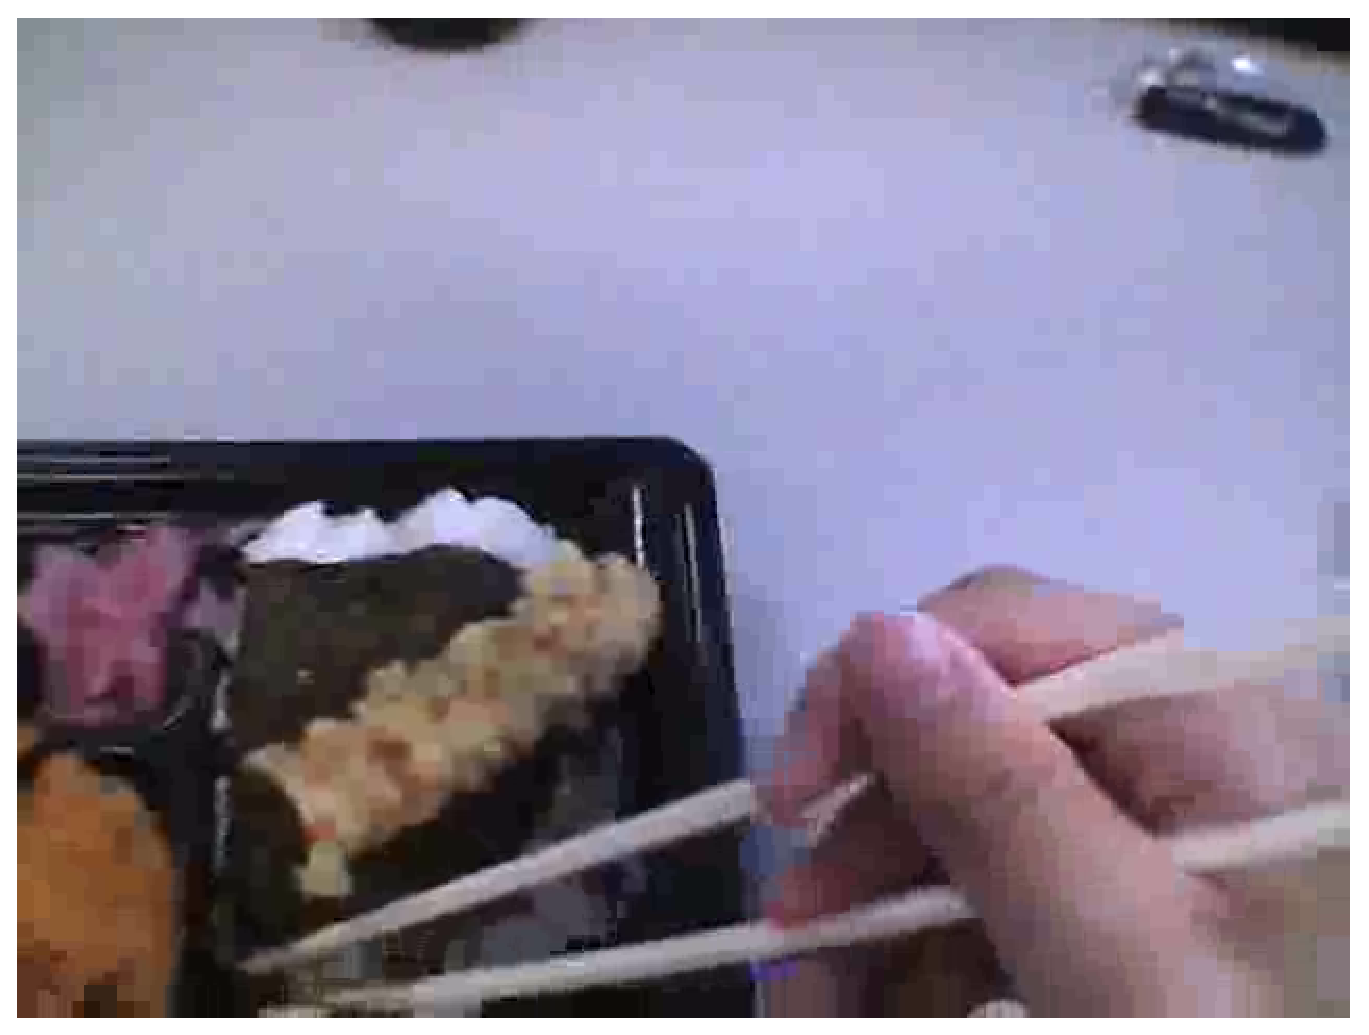
\includegraphics[height=35mm]{figure/fpv_eating.eps}
      \hspace{1.6cm} (a) 食事
      \vspace{3mm}
    \end{center}
  \end{minipage}
%
  \begin{minipage}{0.33\textwidth}
    \begin{center}
      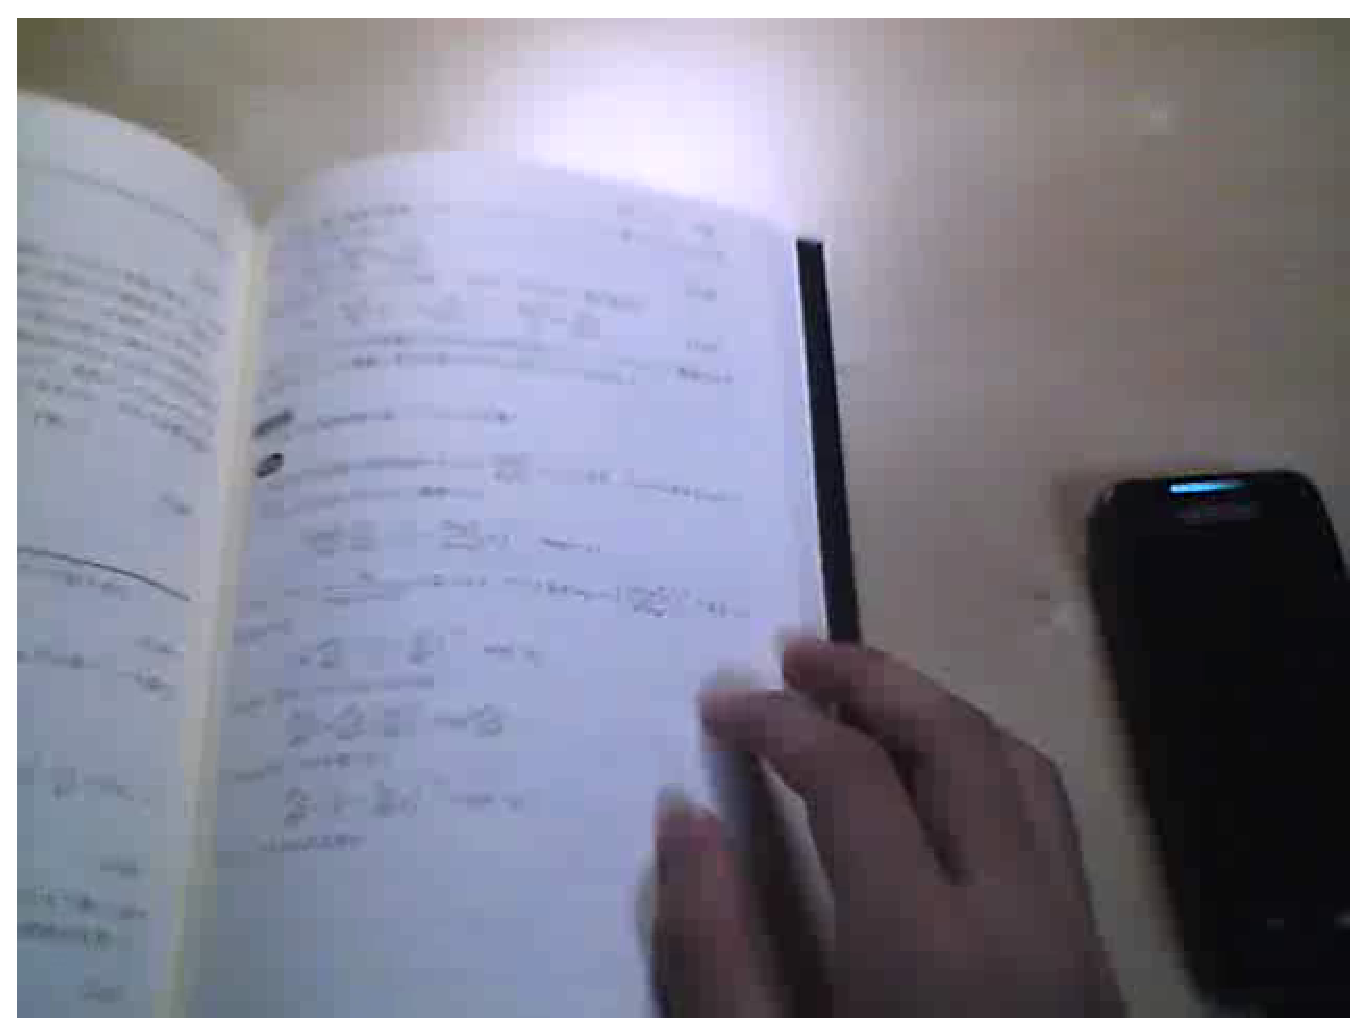
\includegraphics[height=35mm]{figure/fpv_reading.eps}
      \hspace{1.6cm} (b) 読書
      \vspace{3mm}
    \end{center}
  \end{minipage}
%
  \begin{minipage}{0.33\textwidth}
    \begin{center}
      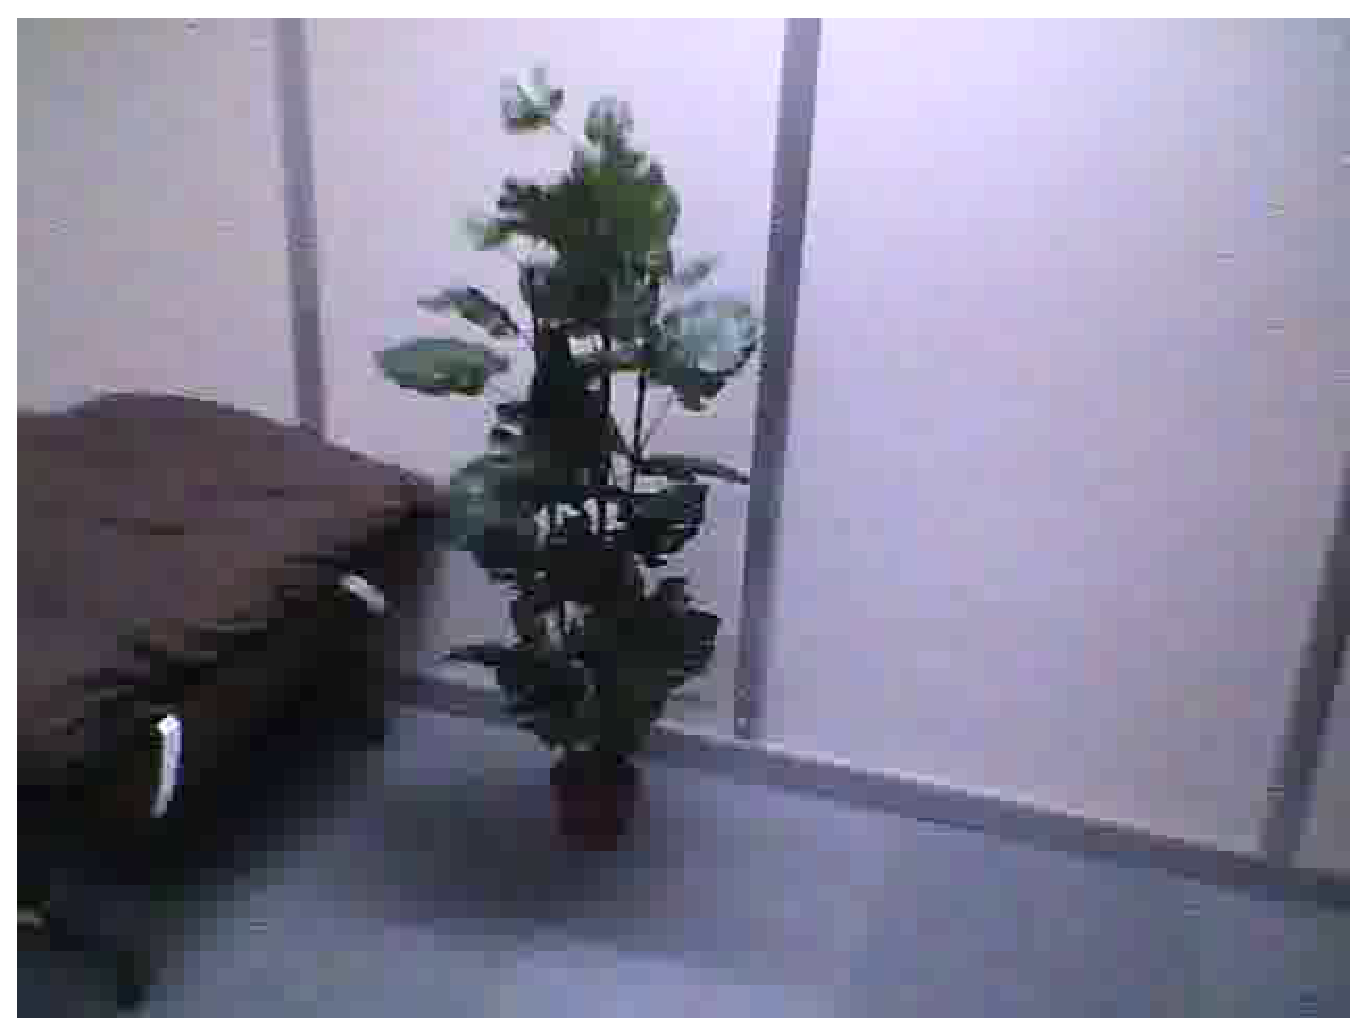
\includegraphics[height=35mm]{figure/fpv_tree.eps}
      \hspace{1.6cm} (c) 植木を注視
      \vspace{3mm}
    \end{center}
  \end{minipage} \\
%
  \begin{minipage}{0.33\textwidth}
    \begin{center}
      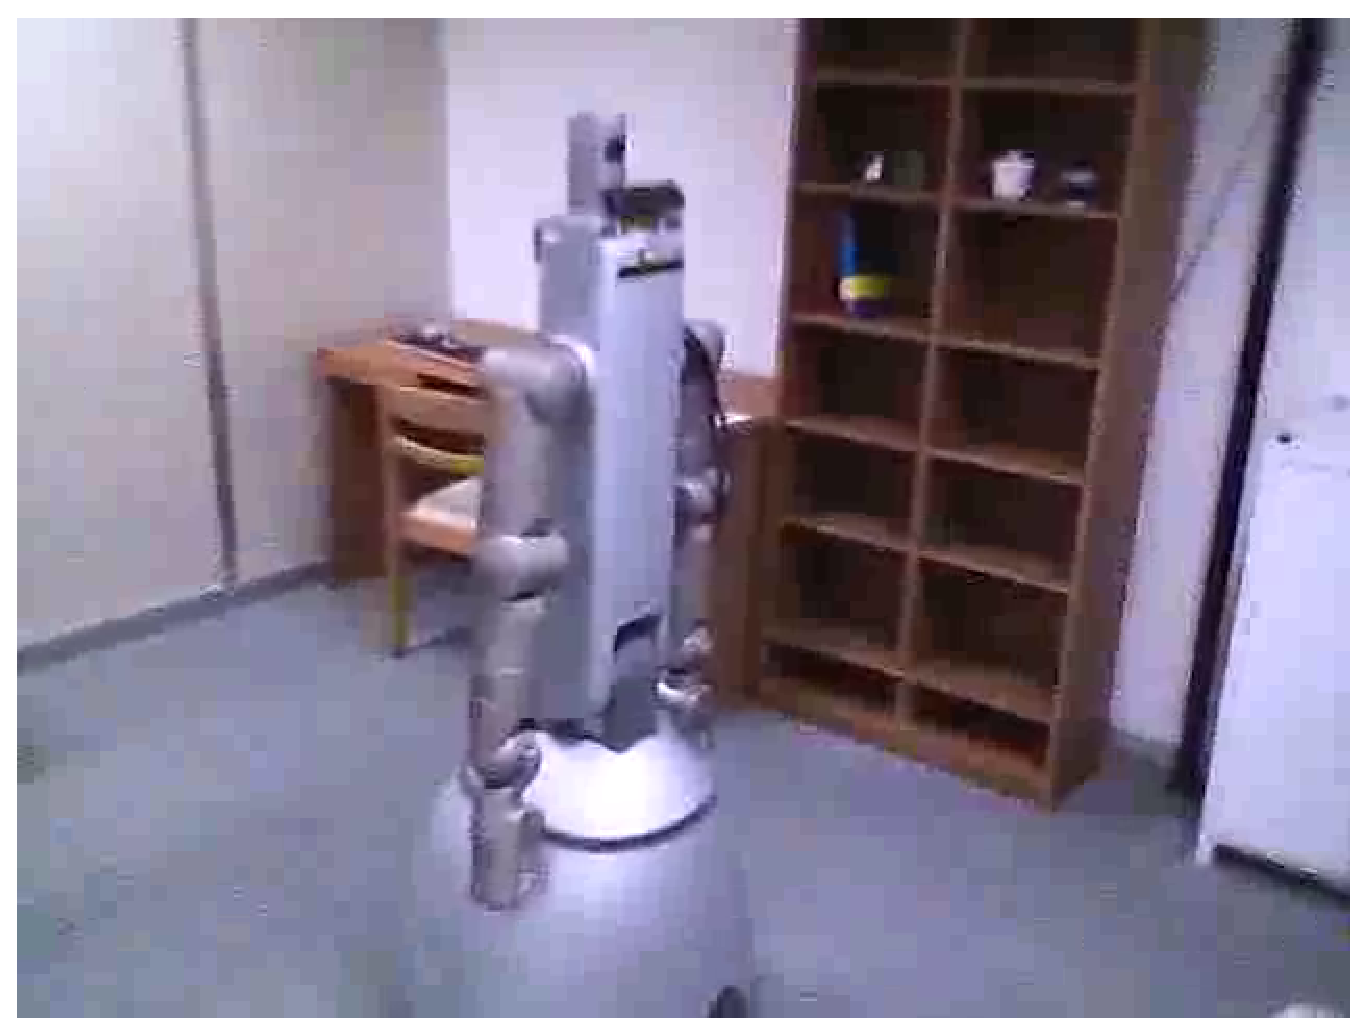
\includegraphics[height=35mm]{figure/fpv_robot.eps}
      \hspace{1.6cm} (d) サービスロボットを注視
    \end{center}
  \end{minipage}
%
  \begin{minipage}{0.33\textwidth}
    \begin{center}
      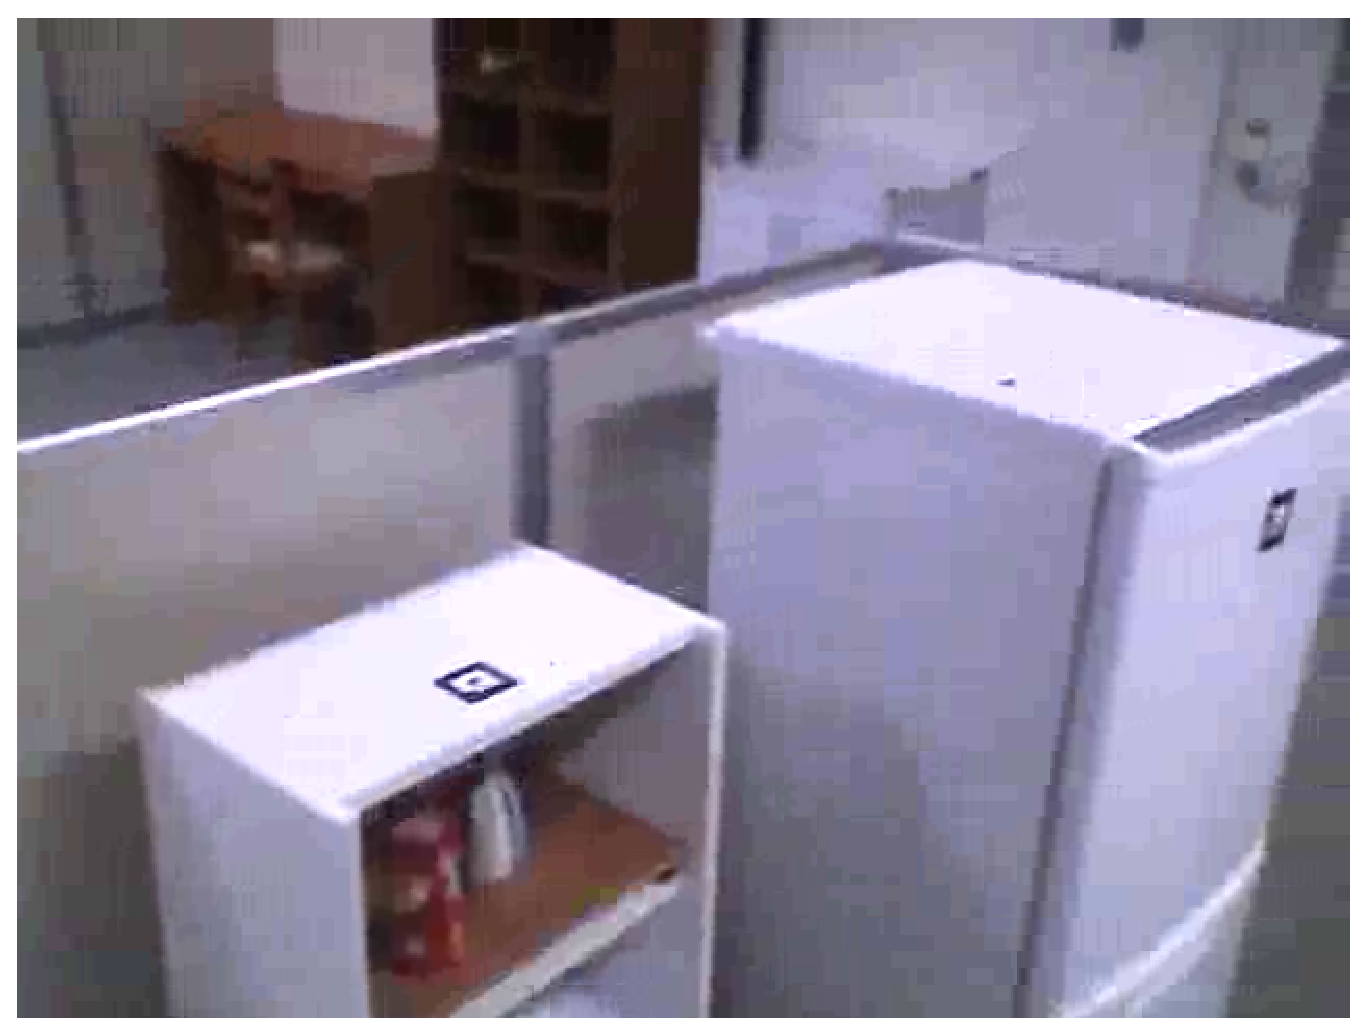
\includegraphics[height=35mm]{figure/fpv_around.eps}
      \hspace{1.6cm} (e) 辺りを見回す
    \end{center}
  \end{minipage}
%
\end{tabular}
\caption{認識対象の行動カテゴリ}
\label{fig:activities}
\end{figure}

これらの行動を認識するためには,それぞれの動画像がどういったユニークな特徴を持つか定量的に記述し,各カテゴリでどういったパターンが現れるか学習する必要がある.
その代表的なアプローチとしては,次の通りである.
%
\begin{enumerate}
\setlength{\itemsep}{-5pt}
\item{学習時}
  \begin{enumerate}
  \setlength{\itemsep}{-5pt}
  \item{多くの学習データから局所特徴を抽出する}
  \item{局所特徴群の統計的分布形状をベクトル表現する}
  \item{求めた特徴ベクトルに正解カテゴリラベルを与えながら,識別器を学習する}
  \end{enumerate}
\item{識別時}
  \begin{enumerate}
  \setlength{\itemsep}{-5pt}
  \item{一つの動画像から局所特徴を抽出する}
  \item{局所特徴群の統計的分布形状をベクトル表現する}
  \item{予め学習した識別器に入力し,識別結果を得る}
  \end{enumerate}
\end{enumerate}

次節以降では,この手順に従って,動画像の時空間変化から局所特徴を得る手法,それら数多くの特徴群を1つの特徴ベクトルにエンコーディングするいくつかの手法,識別器の学習について述べる.

%---------------------------------------------------------------------------------------------------
\section{1人称視点映像データセット}
各行動カテゴリの動画像データは,実際に使用するウェアラブルカメラMoverio BT-200AVから撮影し,複数人の行動パターンを収集した.また,1シーケンスを10秒とし,各カテゴリ50シーケンスの動画像を用意した.画像サイズは$ 320\times240 $,フレームレートを30 fpsとする.

%---------------------------------------------------------------------------------------------------
\section{特徴抽出}
本節では,動画像から局所特徴を抽出する方法について述べる.
%---------------------------------------------------------------------------------------------------
\subsection{Space-Time Interest Points}
一般に,画像から特徴を抽出する場合,特徴点検出と特徴記述の二段階の処理に分けられる.
特徴点検出は,画像空間上のコーナーやエッジなど特徴的な箇所を検出する処理である.
また,特徴記述は,検出した特徴点において,その周辺領域の画素値や輝度の勾配を用いて,どういった特徴を持つか数値的に表す処理である.

一方,動画像の場合は,時系列に並んだ複数の画像から構成されている.
そのため,動画像の特徴として,毎フレームの画像空間上で特徴を計算することもできるが,複数フレーム間の時間変化を検出し,時空間上の局所領域を特徴として表現することもできる.
本研究では,動画像の時空間変化に基いて特徴点を検出する手法として,Laptevが提案したSpace-Time Interest Points (STIP)\cite{stip}を利用した.STIPは,画像空間の代表的なコーナー検出手法であるHarris detectorを時空間に拡張したものである.
STIPより検出した特徴点に関しては,画像空間の輝度勾配に基づいたHistogram of Oriented Gradients (HOG)と特徴点の動きをベクトルで表したHistogram of Optical Flow (HOF)により特徴記述を行う.

\subsection{次元削減}
前節で抽出した局所特徴ベクトルに対し,次元数の削減を行った.次節で局所特徴群のエンコーディングについて述べるが,そのいくつかの手法で求まる最終的な動画像の特徴ベクトルは,局所特徴の次元数に比例した高次元ベクトルとなる.そのため,ここでは計算コストの削減と情報の圧縮を目的として,主成分分析を行った.

主成分分析は,多次元空間上のベクトル群を,元の分布を近似してかつ分散が最大となるような部分空間に射影することで,主要な成分を抽出する手法である.ここでは,学習用の動画像から得る多数の局所特徴$ \bm{x_i} = \left( x_1, \cdots, x_d \right)^{\mathrm{T}} $を並べたパターン集合を$ \bm{X} $とし,部分空間に射影するための変換行列$ \bm{A_{\lambda}} $を求める.
%
\begin{equation}
{
  \bm{X} = \left( \bm{x}_1, \cdots, \bm{x}_N \right)^{\mathrm{T}}
}
\end{equation}

まず,パターン集合$ \bm{X} $の共分散行列$ \bm{\Sigma} $を次式より求める.ただし,$ \bm{M} $は,局所特徴群の平均ベクトルをN個並べたものである.
%
\begin{equation}
{
  \bm{\Sigma} =
  \frac{1}{N}\left(\bm{X}-\bm{M}\right)^{\mathrm{T}}\left(\bm{X}-\bm{M}\right)
}
\end{equation}

次に$ \bm{\Sigma} $の固有値$ \{\lambda_1,\cdots,\lambda_k\} $と,それに対応する固有ベクトル$ \{\bm{p}_1,\cdots,\bm{p}_k\} $を求める.
ここで,固有値の大きいものから順に,$ \tilde{d} $個の固有ベクトルを並べると,上述した変換行列$ \bm{A_{\lambda}} $が求まり,$ d $次元の原特徴ベクトル$ \bm{x} $は次元の少ない特徴ベクトル$ \bm{y} = \left( y_1, \cdots, y_{\tilde{d}} \right)^{\mathrm{T}} $へ変換される.すなわち,$ \bm{\Sigma} $の固有ベクトルが部分空間を張る基底となり,各基底における分散の大きさが固有値で表される.全ての固有ベクトルを基底とすれば,部分空間における特徴ベクトルの分散は最大となる.
%
\begin{equation}
{
  \bm{y} = \bm{A_{\lambda}}^{\mathrm{T}}\bm{x}
}
\end{equation}

また,大きい順にいくつかの固有値を加算した値が,全ての固有値の和に対して占める割合を累積寄与率と呼び,元の局所特徴ベクトルの分布をどれだけ近似できるかを示す.本研究では,累積寄与率95\%までの固有ベクトルを利用し,次元削減を行った.

\newpage
%---------------------------------------------------------------------------------------------------
\section{局所特徴群のエンコーディング}
これまで,画像から得られる多数の局所特徴群に対し,その統計量を利用した特徴表現手法が数多く提案されてきた.本研究では,局所特徴のエンコーディング手法としては一般的なBag of Visual Words\cite{bovw}に加えて,より高次の統計量を利用するFisher Vector\cite{fisher_vector},Vector of Locally Aggregated Descriptors (VLAD)\cite{vlad}の3手法を動画像に適用し,それぞれの識別性能,計算時間を比較した.また,各手法の計算には,コンピュータビジョンに関する多数のアルゴリズムを実装したオープンソースライブラリVLFeat\footnote{http://www.vlfeat.org}を利用し,クラスタリングや正規化処理の手順はこれに準拠する.

%---------------------------------------------------------------------------------------------------
\subsection{Bag of Visual Words}
Bag of Visual Words\cite{bovw}は,統計的文書表現手法であるBag of Words modelのアプローチを類推し,コンピュータビジョンの分野で画像に適用したものである.Bag of Wordsでは,文脈を無視し,代表的な単語の出現頻度により文書を表現することで,効率的な文書分類を可能にした.同様に,Bag of Visual Wordsでは,予め多くの学習画像から決定した代表的な局所特徴をVisual Wordsと呼び,これらを並べた記述子(Visual Codebook)に従って,画像を一つの特徴ベクトルで表現する.多数の局所特徴を一つの特徴ベクトルにエンコーディングする手法として,Bag of Visual Wordsは代表的なものであり,一般物体認識の分野で広く用いられている.本研究では,動画像から抽出した局所特徴に対して同様の手順を適用することで,効率的な動画像の特徴表現を図る.

Bag of Visual Wordsの具体的な計算手順について述べる.まず,エンコーディングを行う前の学習段階としてVisual Wordsを作成するために,学習セットから多数の局所特徴を抽出する.さらに,抽出された局所特徴群に対してクラスタリングを行い,各クラスタの中心をVisual Wordsとする.本研究では,代表的なクラスタリング手法であるk-means法を適用した.求まったVisual Wordsを並べ,Visual Codebook $ \bm{C} = (c_1, c_2, \cdots, c_k) $を作成する.

次に,学習したVisual Codebookに基づいて,入力動画像から得られる局所特徴群のエンコーディングを行う.抽出された局所特徴は,それぞれ特徴空間上で最近傍となるVisual wordへ割り当てる.この際,各Visual Wordsにおいて割り当てられた局所特徴の数をカウントすることで,Visual Wordsのヒストグラムが作成される.ただし,ここで作成されるヒストグラムは局所特徴の抽出数に依存し,過学習に陥る可能性がある他,フレーム数の異なる入力動画像に対して正しく汎化できない.そのため,求まったヒストグラムに対し,正規化を施す.本研究では,$ L^2 $正規化を適用した.$ L^2 $正規化を行う場合,Visual Wordsをビンとしたヒストグラムを$ \bm{H} =  (h_1, h_2, \cdots, h_k)^{\mathrm{T}} $,正規化処理後の最終的な特徴ベクトルを$ \bm{v} =  (v_1, v_2, \cdots, v_k)^{\mathrm{T}} $とすると,各要素$ h_i $はベクトル$ \bm{H} $の$ L^2 $ノルムにより除算される.
%
\begin{equation}
{ v_i = \frac{h_i}{\lVert{\bm{H}}\rVert_2} = \frac{h_i}{ \sqrt{\sum_{j=1}^{k} h_j^2} } }
\end{equation}

以上のようにして求まったベクトル$ \bm{v} $を,動画像を表現する特徴ベクトルとする.最終的な特徴ベクトルの次元は,k-means法で設定したクラスタ数$ k $に一致する.
%
\begin{figure}[htbp]
\begin{tabular}{ccc}
%
 \begin{minipage}{0.33\textwidth}
  \begin{center}
   \includegraphics[height=40mm]{figure/bovw_1.eps}
   \hspace{1.6cm} (1) 局所特徴抽出(学習時)
  \end{center}
 \end{minipage}
%
 \begin{minipage}{0.33\textwidth}
  \begin{center}
   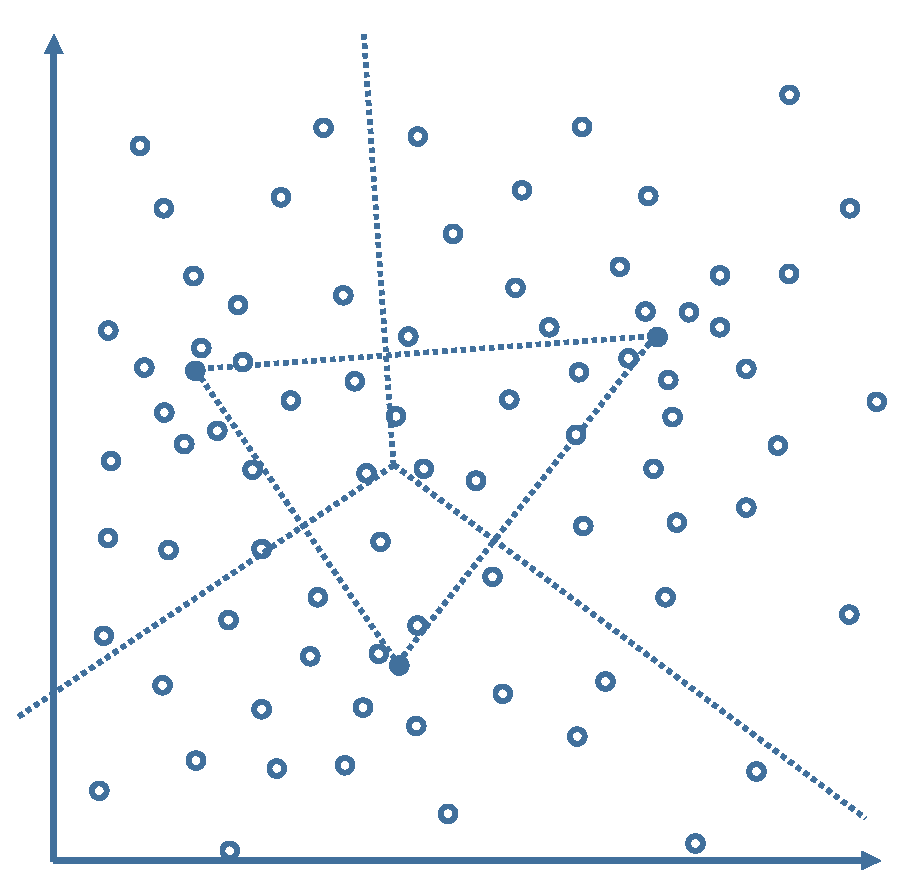
\includegraphics[height=40mm]{figure/bovw_2.eps}
   \hspace{1.6cm} (2) K-meansクラスタリング
  \end{center}
 \end{minipage}
%
 \begin{minipage}{0.33\textwidth}
  \begin{center}
   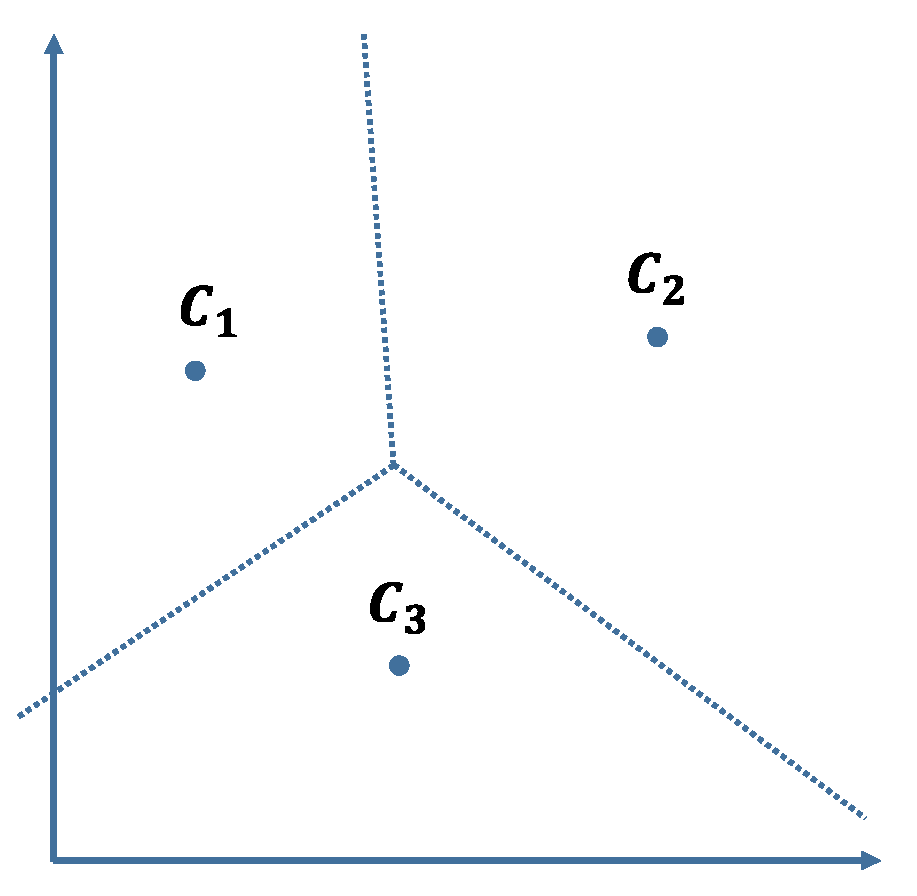
\includegraphics[height=40mm]{figure/bovw_3.eps}
   \hspace{1.6cm} (3) Visual Words (k-means)作成
  \end{center}
 \end{minipage} \\
%
 \begin{minipage}{0.33\textwidth}
  \begin{center}
   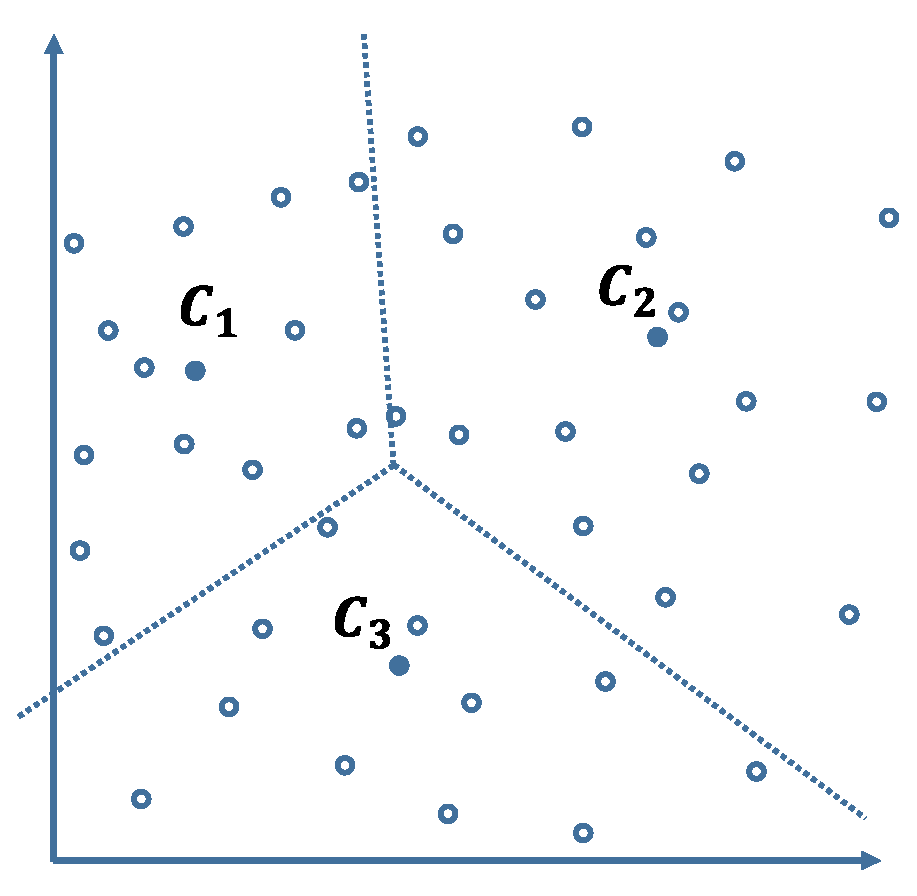
\includegraphics[height=40mm]{figure/bovw_4.eps}
   \hspace{1.6cm} (4) 局所特徴抽出(識別時)
  \end{center}
 \end{minipage}
%
 \begin{minipage}{0.33\textwidth}
  \begin{center}
   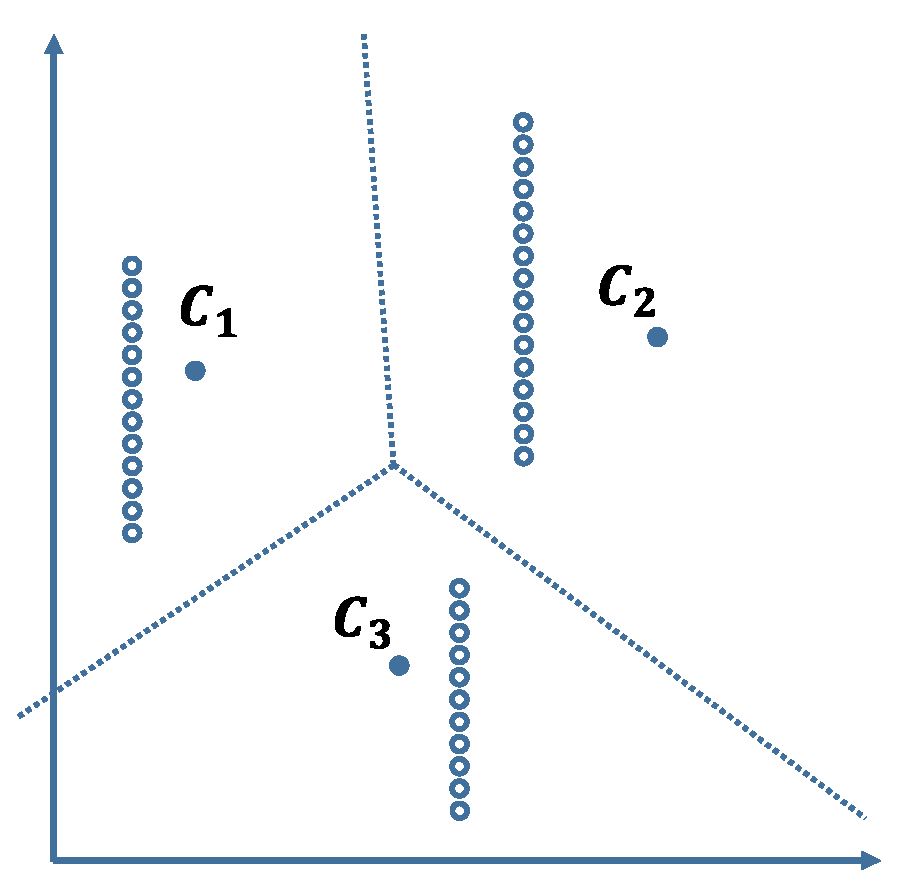
\includegraphics[height=40mm]{figure/bovw_5.eps}
   \hspace{1.6cm} (5) 局所特徴の数をカウント
  \end{center}
 \end{minipage}
%
\end{tabular}
\caption{Bag of Visual Wordsエンコーディング手順}
\label{fig:bag_of_visual_words}
\end{figure}
%
\newpage
%
%---------------------------------------------------------------------------------------------------
\subsection{Fisher Vector}
Fisher Vectorは,2007年にF. Perronninらによって提案された\cite{fisher_vector}.従来の一般的なエンコーディング手法であるBag of Visual Wordsでは,多数得られる局所特徴をいずれかのVisual wordに割り当てることでベクトル量子化を行い,各Visual Wordsの出現頻度を利用した.しかし,Visual Wordsの出現頻度のみで局所特徴の分布形状を良く表すためには,量子化誤差を少なくするために,多くのVisual Wordsを用意する必要がある.もしくは,識別する際に,カーネル法を用いた高次元空間への写像を検討しなければ,高い識別性能は期待できず,これらは計算コストの増大が問題となる.
Fisher Vectorは,こういった問題の解決策として,Fisher Kernel\cite{fisher_vector2}を画像分類に応用した.以下に,その概要を示す.

一般的に,クラス分類問題の主なアプローチとして,生成モデルと識別モデルが挙げられる.生成モデルは,異なるデータサイズを扱える利点があるが,一方で,識別モデルはクラス識別そのものに着目しているため,より良い識別結果を示すことが知られている.Fisher Kernelは,生成モデルからカーネル関数を定義する枠組みであり,このカーネルを用いて識別モデルのアプローチを取ることで,両者の恩恵を受けることができる.

まず,画像から抽出される局所特徴が$ \bm{\theta} = \{\bm{\theta_m}, m=1,2,\cdots,M\}$をパラメータとする確率密度関数$ p(\bm{x}|\bm{\theta}) $に従って生成されるものと仮定する.さらに,仮定したモデルに対して,画像から抽出される局所特徴分布$ \bm{X} = \{\bm{x_t}, t=1,2,\cdots,T\} $が与えられたとすると,それぞれの局所特徴$ \bm{x_t} $における尤度が$ p(\bm{x_t}|\bm{\theta}) $により計算される.それら尤度を最大化するように$ \bm{\theta} $を決めれば,局所特徴分布$ \bm{X} $に最もフィットするモデルを求めることができる.すなわち,$ \bm{x_t} $がそれぞれ独立に生起するものと仮定すれば,次式を最大化すればよい.
%
\begin{equation}
\label{eq:likelihood}
{ p(\bm{X}|\bm{\theta}) = \prod_{t=1}^{T} p(\bm{x_t}|\bm{\theta}) }
\end{equation}

Fisher Kernelでは,ここで次のスコア関数$ \bm{G}_{\bm{X}} $を考える.
%
\begin{equation}
\label{eq:fisher_score}
{
\bm{G}_{\bm{X}} 
= \frac{1}{T} \sum_{t=1}^{T} \nabla_{\bm{\theta}} \log p(\bm{x_t}|\bm{\theta}) 
= \frac{1}{T} \nabla_{\bm{\theta}} \log p(\bm{X}|\bm{\theta}) 
}
\end{equation}

$ \bm{G}_{\bm{X}} $は,$ \bm{X} $に関する対数尤度の勾配を計算したもので,Fisher scoreと呼ばれる.仮定した生成モデルを,与えられた局所特徴分布$ \bm{X} $に最も良くフィットさせるために,それぞれのパラメータ$ \bm{\theta} $をどの方向に変化させるべきかを示す.また,$ \bm{G}_{\bm{X}} $の次元は,局所特徴の数Tに依らず,生成モデルのパラメータ数で決まるため,$ \bm{X} $の分布形状を記述する一種の特徴ベクトルとして利用することができる.これが,不定量のデータ$ \bm{X} $を,特定のサイズのベクトルへエンコーディングする原理であり,生成モデルによるカーネル定義の最大の利点である.

また,特徴ベクトルとして,実際に内積を用いた識別器に入力するために,標準偏差によるスケーリング(whitening)を行う必要がある.そのために,次式のFisher情報行列を計算する.
%
\begin{equation}
{ \bm{F_\theta} = \bm{E_X} \left[ \bm{G}_{\bm{X}}\bm{G}_{\bm{X}}^{\mathrm{T}} \right] }
\end{equation}

Fisher情報行列は,Fisher scoreに関する共分散を表し,その平方根で除算を行うことで,次のベクトルを得る.
%
\begin{equation}
\label{eq:fisher_vector}
{
\bm{g}_{\bm{X}} 
= \bm{F_\theta}^{-1/2}\bm{G}_{\bm{X}} 
= \frac{1}{T} \bm{F_\theta}^{-1/2} \nabla_{\bm{\theta}} \log p(\bm{X}|\bm{\theta})
}
\end{equation}

上記ベクトル$ \bm{g}_{\bm{X}} $がFisher Vectorであり,Fisher Kernelは,Fisher Vectorの単純な内積で表される.すなわち,$ \bm{g}_{\bm{X}} $を画像の特徴ベクトルとして利用することができれば,計算コストの少ない線形カーネルに置き換えて識別器を学習することができる.
%
\begin{equation}
{
\bm{K}(\bm{X},\bm{Y}) 
= {{\bm{G}_{\bm{X}}}^{\mathrm{T}}}{\bm{F_\theta}^{-1}}{\bm{G}_{\bm{Y}}}
= {\bm{g}_{\bm{X}}}^{\mathrm{T}} \bm{g}_{\bm{Y}} 
}
\end{equation}

次に,実際にモデルを当てはめて,Fisher Vectorの具体的なベクトル要素について述べる.Fisher Vectorは,確率密度関数のモデルとしてGaussian Mixture Model (GMM)を考え,混合する各ガウス分布をVisual Wordsと捉える.すなわち,パラメータ$ \bm{\theta} $は,GMMを構成するN個のガウス分布$ p_i(\bm{x}|\bm{\theta}) $の重み$ w_i $,平均ベクトル$ \bm{\mu_i} $,共分散行列$ \bm{\Sigma_i} $で構成される.
%
\begin{equation}
\label{eq:gmm}
{
p(\bm{X}|\bm{\theta}) = \sum_{i=1}^{N} w_i p_i(\bm{X}|\bm{\theta}) 
= \sum_{i=1}^{N} w_i \frac{1}{ (2\pi)^{D/2}{\lvert{\bm{\Sigma_i}}\rvert}^{1/2} }{exp\left\{-\frac{1}{2}(\bm{X}-\bm{\mu_i})^{\mathrm{T}}\bm{\Sigma_i^{-1}}(\bm{X}-\bm{\mu_i})\right\}} 
}
\end{equation}
%
\begin{equation}
\label{eq:theta}
{
  \bm{\theta} = (\bm{\theta_1},\cdots,\bm{\theta_M}) 
  = (w_1,\cdots,w_N,\bm{\mu_1},\cdots,\bm{\mu_N},\bm{\Sigma_1},\cdots,\bm{\Sigma_N}) 
}
\end{equation}

ただし,計算コストを削減するため,共分散行列$ \bm{\Sigma_i} $は対角行列と近似し,以降では分散ベクトル$ \bm{\sigma_i} $と表す.従って,(\ref{eq:fisher_vector})のFisher Vectorの各要素は次のようになる.
%
\begin{equation}
{
  \bm{g}_{\bm{X}} 
  = \frac{1}{T} \bm{F_\theta}^{-1/2} \left\{
    \frac{\partial \log p(\bm{X}|\theta)}{\partial w_2}, 
    \cdots, 
    \frac{\partial \log p(\bm{X}|\theta)}{\partial w_N}, 
    \frac{\partial \log p(\bm{X}|\theta)}{\partial \bm{\mu_1}}, 
    \cdots, 
    \frac{\partial \log p(\bm{X}|\theta)}{\partial \bm{\mu_N}}, 
    \frac{\partial \log p(\bm{X}|\theta)}{\partial \bm{\sigma_1}}, 
    \cdots, 
    \frac{\partial \log p(\bm{X}|\theta)}{\partial \bm{\sigma_N}}
  \right\}^{\mathrm{T}}
}
\end{equation}
%
\begin{equation}
\label{eq:weight}
{
  \frac{\partial \log p(\bm{X}|\theta)}{\partial w_i}
  = \sum_{t=1}^{T} \left\{ \frac{\gamma_t(i)}{w_i}-\frac{\gamma_t(1)}{w_1} \right\}  (i \geq 2)
}
\end{equation}
%
\begin{equation}
{
  \frac{\partial \log p(\bm{X}|\theta)}{\partial \bm{\mu_i}}
  = \sum_{t=1}^{T} \gamma_t(i) \left( \frac{\bm{x_t}-\bm{\mu_i}}{\bm{\sigma_i}^2} \right)
}
\end{equation}
%
\begin{equation}
{
  \frac{\partial \log p(\bm{X}|\theta)}{\partial \bm{\sigma_i}}, 
  = \sum_{t=1}^{T} \gamma_t(i) \left\{ \frac{(\bm{x_t}-\bm{\mu_i})^2}{\bm{\sigma_i}^3}-\frac{1}{\bm{\sigma_i}} \right\}
}
\end{equation}

$ \gamma_t(i) $は,$ \bm{x_t} $がi番目のガウス分布に存在する確率(事後確率)である.
%
\begin{equation}
{
  \gamma_t(i)
  = \frac{w_i p_i(\bm{x}|\bm{\theta})}{\sum_{j=1}^{N} w_j p_i(\bm{x}|\bm{\theta})}
}
\end{equation}

また,計算を簡単にするため,Fisher情報行列$ \bm{F_\theta} $は対角行列とし,(\ref{eq:weight})の重み$ w_i $に関する勾配は,特徴としての寄与が小さいため,無視する.最終的なFisher Vectorは次式となる.
%
\begin{equation}
{
  \bm{g}_{\bm{X}} 
  = \left\{
  \bm{g_{\mu_1}},
  \cdots,
  \bm{g_{\mu_N}},
  \bm{g_{\sigma_1}},
  \cdots,
  \bm{g_{\sigma_N}},
  \right\}^{\mathrm{T}}
}
\end{equation}
%
\begin{equation}
\label{eq:mean}
{
  \bm{g_{\mu_i}}
  = \frac{1}{T\sqrt{w_i}} \sum_{t=1}^{T} \gamma_t(i) \left( \frac{\bm{x_t}-\bm{\mu_i}}{\bm{\sigma_i}} \right)
}
\end{equation}
%
\begin{equation}
\label{eq:variance}
{
  \bm{g_{\sigma_i}}
  = \frac{1}{T\sqrt{2w_i}} \sum_{t=1}^{T} \gamma_t(i) \left\{ \frac{(\bm{x_t}-\bm{\mu_i})^2}{\bm{\sigma_i}^2}-1 \right\}
}
\end{equation}

求まったFisher Vectorは,$ \bm{g_{\mu_i}} $と$ \bm{g_{\sigma_i}} $がそれぞれ$ \bm{x_t} $と同等の次元を持つため,全体としては局所特徴の次元数$ D $とGMMの混合数$ N $に対して,$ 2\times{D}\times{N} $の次元を持つ.また,(\ref{eq:mean})と(\ref{eq:variance})は,それぞれ$ \bm{x_t} $に関して1次と2次の統計量を表す.このように,0次の統計量(出現回数)のみを扱った従来のBag of Visual Wordsに比べ,同じVisual Words数でもより多くの統計情報を抽出することができる.本研究では,動画像から得られる局所特徴に対して,Fisher Vectorを適用する.

以上を踏まえて,Fisher Vectorのエンコーディングの流れを述べる.まず,予め学習セットから多くの局所特徴を抽出し,(\ref{eq:gmm})の尤度を最大とするGMMのパラメータ$ \bm{\theta} = (w_1,\cdots,w_N,\bm{\mu_1},\cdots,\bm{\mu_N},\bm{\Sigma_1},\cdots,\bm{\Sigma_N}) $を推定する.これにより,Visual Wordsとなる各ガウス分布が形成され,Visual Codebookが求まる.次に,入力動画像から得られる局所特徴のエンコーディングを行う.まず,対象の動画像から局所特徴を抽出し,続いて学習したGMMのパラメータに基いて,(\ref{eq:mean})と(\ref{eq:variance})を計算する.最終的に,両者を結合したベクトルを動画像の特徴ベクトルとすることで,学習したGMMの平均と分散に関するパラメータをどのように変化させれば入力動画像の局所特徴分布にフィットするか表現される.

\begin{figure}[htbp]
\begin{tabular}{ccc}
%
 \begin{minipage}{0.33\textwidth}
  \begin{center}
   \includegraphics[height=40mm]{figure/fisher_1.eps}
   \hspace{1.6cm} (1) 局所特徴抽出(学習時)
  \end{center}
 \end{minipage}
%
 \begin{minipage}{0.33\textwidth}
  \begin{center}
   \includegraphics[height=40mm]{figure/fisher_2.eps}
   \hspace{1.6cm} (2) GMMフィッティング
  \end{center}
 \end{minipage}
%
 \begin{minipage}{0.33\textwidth}
  \begin{center}
   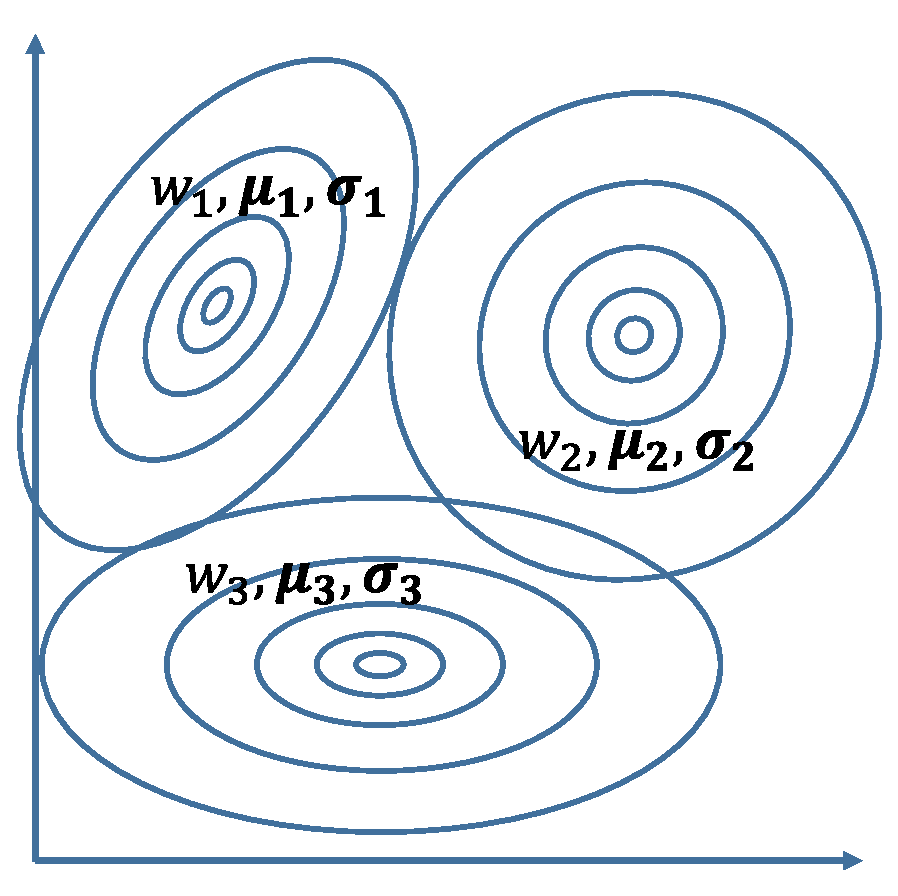
\includegraphics[height=40mm]{figure/fisher_3.eps}
   \hspace{1.6cm} (3) Visual Codebook作成
  \end{center}
 \end{minipage} \\
%
 \begin{minipage}{0.33\textwidth}
  \begin{center}
   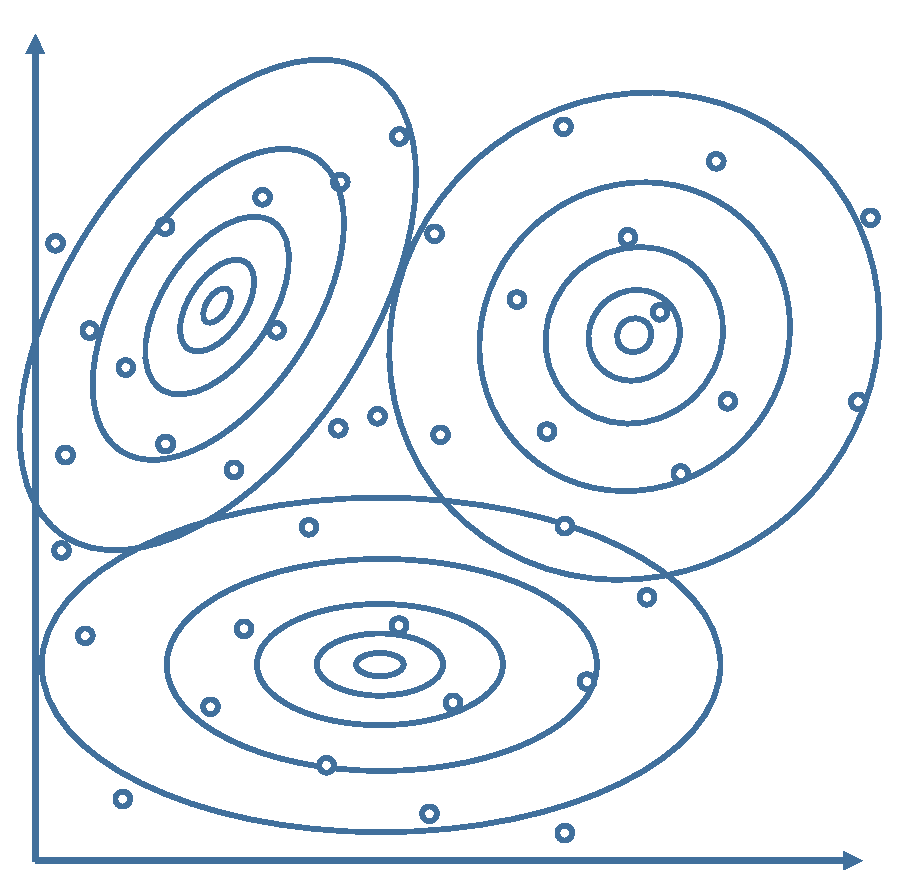
\includegraphics[height=40mm]{figure/fisher_4.eps}
   \hspace{1.6cm} (4) 局所特徴抽出(識別時)
  \end{center}
 \end{minipage}
%
 \begin{minipage}{0.33\textwidth}
  \begin{center}
   \includegraphics[height=40mm]{figure/fisher_5.eps}
   \hspace{1.6cm} (5) 対数尤度の勾配を計算
  \end{center}
 \end{minipage}
%
 \begin{minipage}{0.33\textwidth}
  \begin{center}
   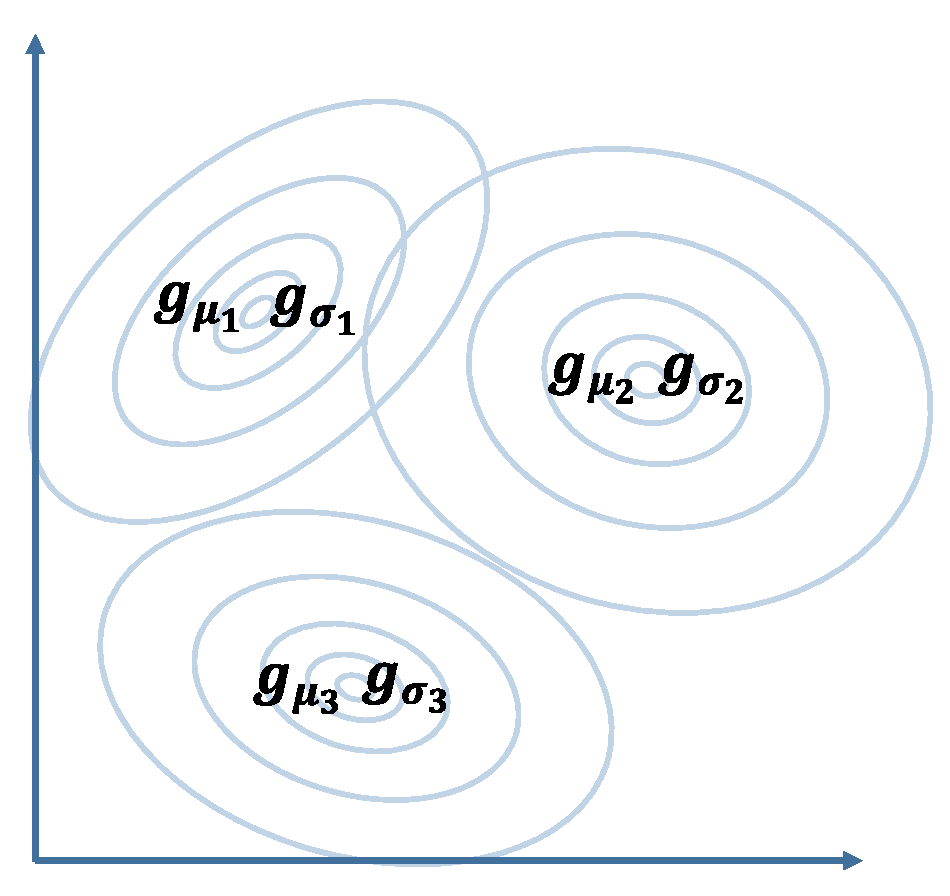
\includegraphics[height=40mm]{figure/fisher_6.eps}
   \hspace{1.6cm} (5) 特徴ベクトル化
  \end{center}
 \end{minipage}
%
\end{tabular}
\caption{Fisher Vectorエンコーディング手順}
\label{fig:fisher_encoding}
\end{figure}

さらに,求まったFisher Vectorに対して,正規化を行う.適用する正規化手法は,F. Perronninらが従来のFisher Vectorに対する改良手法を発表した文献\cite{fisher_vector3}に従って,まず,平方根によるパワー正規化を行い,続いて$ L^2 $正規化を行った.

平方根によるパワー正規化は,Fisher Vectorの各要素$ g_i $に次式を適用することで行う.
% 平方根によるパワー正規化
\begin{equation}
{ {g_i}' = sign(g_i)\sqrt{\lvert{g_i}\rvert} }
\end{equation}

$ L^2 $正規化は,全体の$ L^2 $ノルムで各要素$ {g_i}' $を除算する.

%---------------------------------------------------------------------------------------------------
\subsection{Vector of Locally Aggregated Descriptors}
Vector of Locally Aggregated Descriptors (VLAD)は,2010年にH. Jegouらによって提案された\cite{vlad}.前項のFisher Vectorでは,局所特徴分布から高次統計量を抽出すべく,Gaussian Mixture Modelをフィットさせ,各ガウス分布の平均と分散に基づく特徴ベクトルを導いた.これに対してVLADでは,クラスタ毎に,その平均(centroids)を基準とした局所特徴の分布をベクトルで表し,1次の統計量を抽出する.さらに,最終的に各クラスタのベクトルを並べることで,全体として一つの特徴ベクトルを生成する.このようにして求まったベクトルは,Fisher Vectorの平均に関する要素に相当し,Fisher kernelを簡易化したものと見なすことができる.

VLADの具体的な計算手順について述べる.まず,Bag of Visual Wordsと同様に,学習セットから多くの局所特徴を抽出し,k-means法によるクラスタリングを行う.さらに,各クラスタの中心をVisual WordsとしたVisual Codebook $ \bm{C} = (c_1, c_2, \cdots, c_k) $を作成する.エンコーディング対象の動画像に対しては,同様に局所特徴を抽出し,最近傍のVisual wordに割り当てる.VLADでは,続いて,各Visual Words $ \bm{c_i} $毎に,割り当てられた局所特徴ベクトル$ \bm{x_j} $との差分 $ \bm{x_j} - \bm{c_i} $の総和を取り,次式のベクトル$ \bm{v_i} $を計算する.

\begin{equation}
{ \bm{v_i} = \sum_{j=1}^{N} (\bm{x_j} - \bm{c_i}) }
\end{equation}

ここで,Nは割り当てられた局所特徴の数である.VLADの最大の特徴は,このベクトル$ \bm{v_i} $が,各クラスタにおける局所特徴の分布形状を表現することである.全体としての特徴ベクトルは,これらを並べた次のベクトル$ \bm{v} $で決定され,局所特徴ベクトルの次元$ d $とクラスタ数$ k $に対して,$ d \times k $の次元を持つ.
% VLAD descriptor
\begin{equation}
{ \bm{v} = (\bm{v_1}, \bm{v_2}, \cdots, \bm{v_k})^{\mathrm{T}} }
\end{equation}
%
\begin{figure}[htbp]
\begin{tabular}{ccc}
%
 \begin{minipage}{0.33\textwidth}
  \begin{center}
   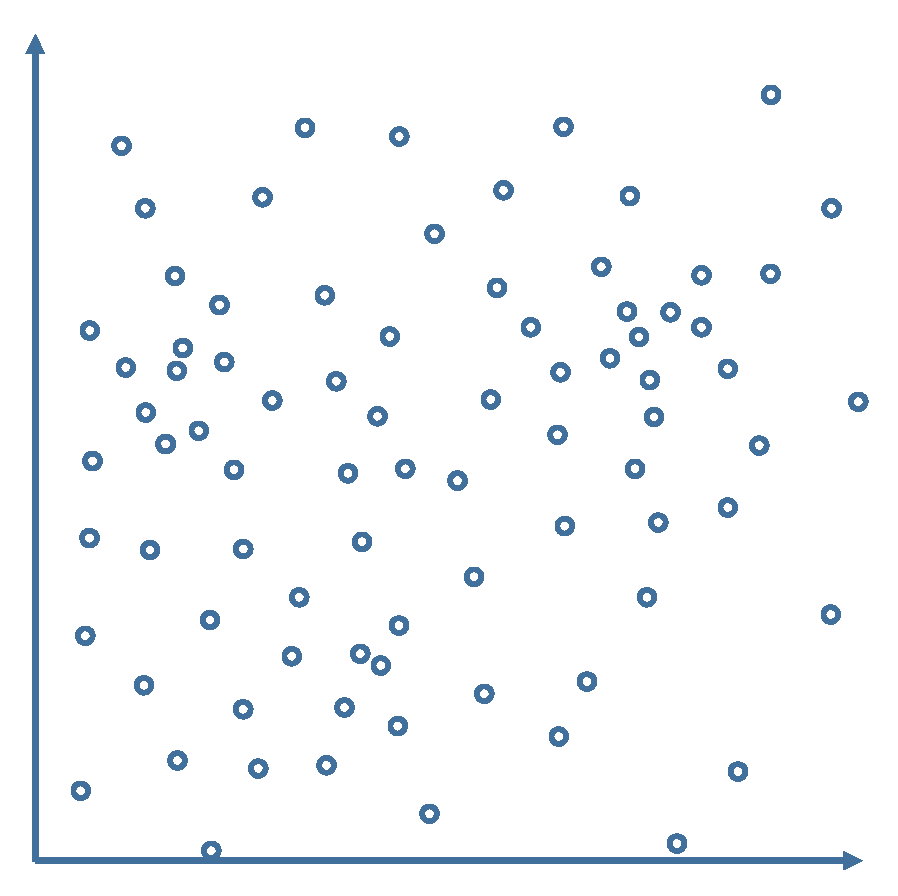
\includegraphics[height=40mm]{figure/vlad_1.eps}
   \hspace{1.6cm} (1) 局所特徴抽出(学習時)
  \end{center}
 \end{minipage}
%
 \begin{minipage}{0.33\textwidth}
  \begin{center}
   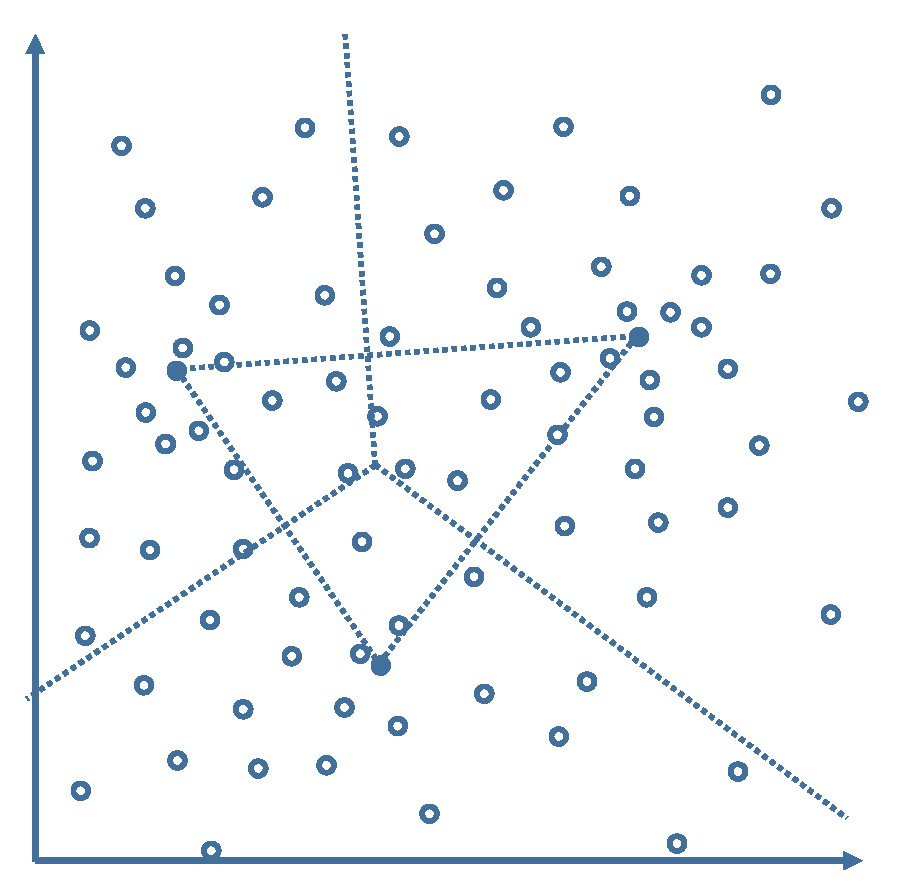
\includegraphics[height=40mm]{figure/vlad_2.eps}
   \hspace{1.6cm} (2) K-meansクラスタリング
  \end{center}
 \end{minipage}
%
 \begin{minipage}{0.33\textwidth}
  \begin{center}
   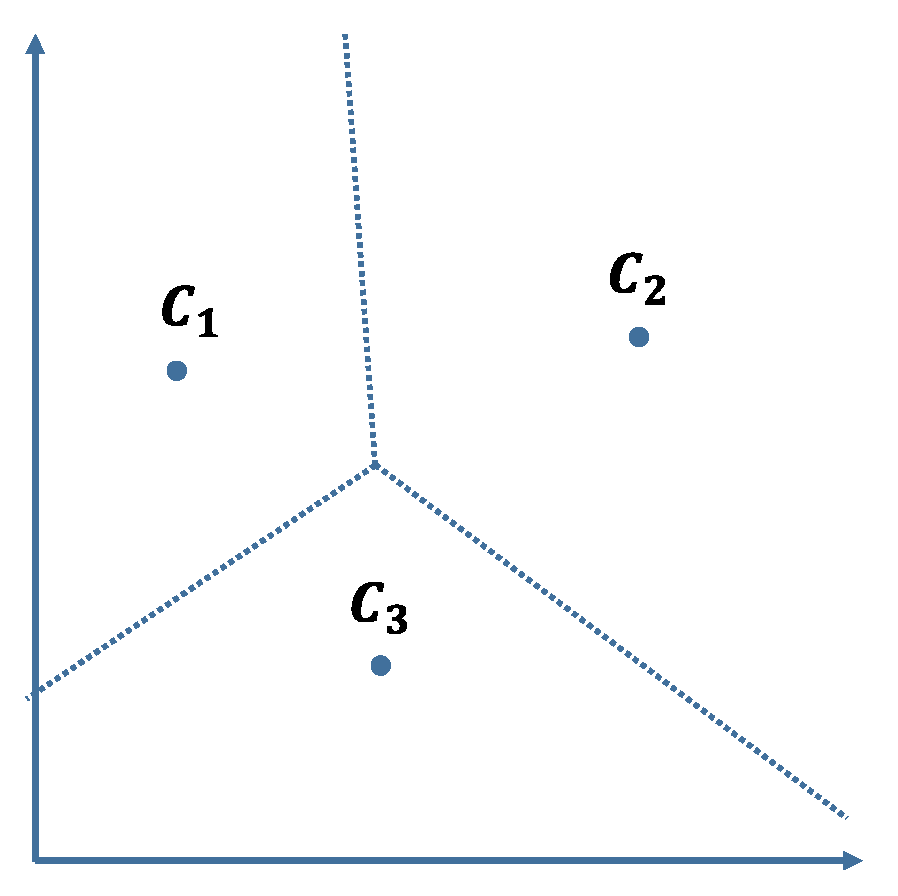
\includegraphics[height=40mm]{figure/vlad_3.eps}
   \hspace{1.6cm} (3) Visual Words (k-means)生成
  \end{center}
 \end{minipage} \\
%
 \begin{minipage}{0.33\textwidth}
  \begin{center}
   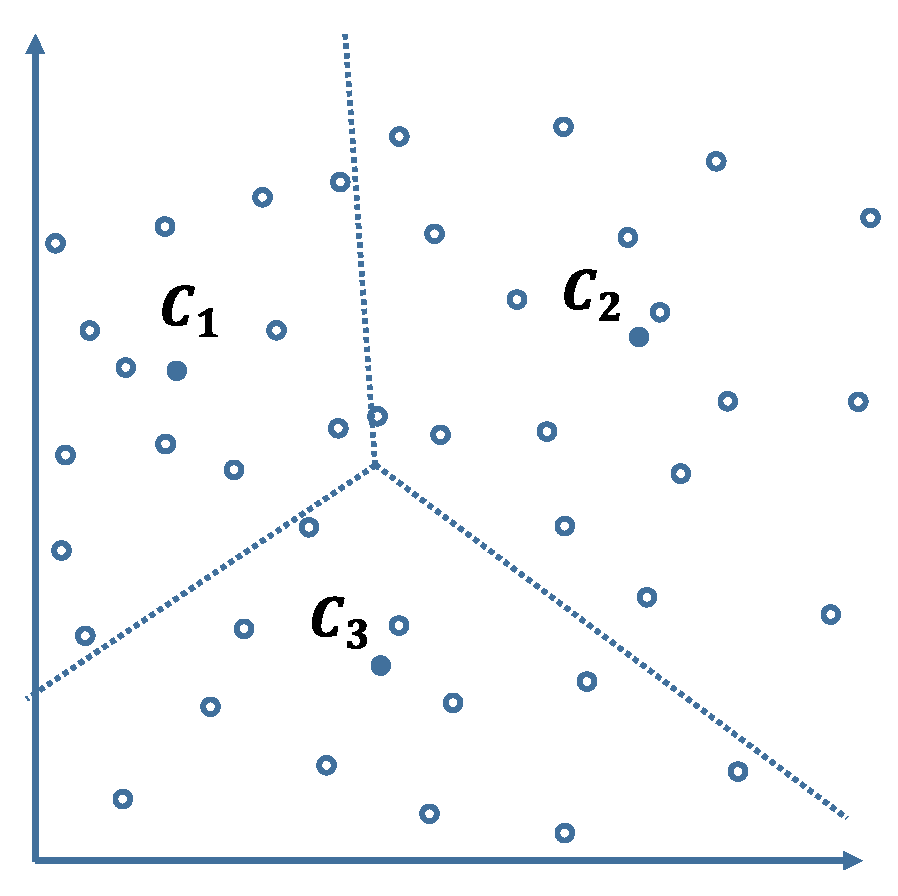
\includegraphics[height=40mm]{figure/vlad_4.eps}
   \hspace{1.6cm} (4) 局所特徴抽出(識別時)
  \end{center}
 \end{minipage}
%
 \begin{minipage}{0.33\textwidth}
  \begin{center}
   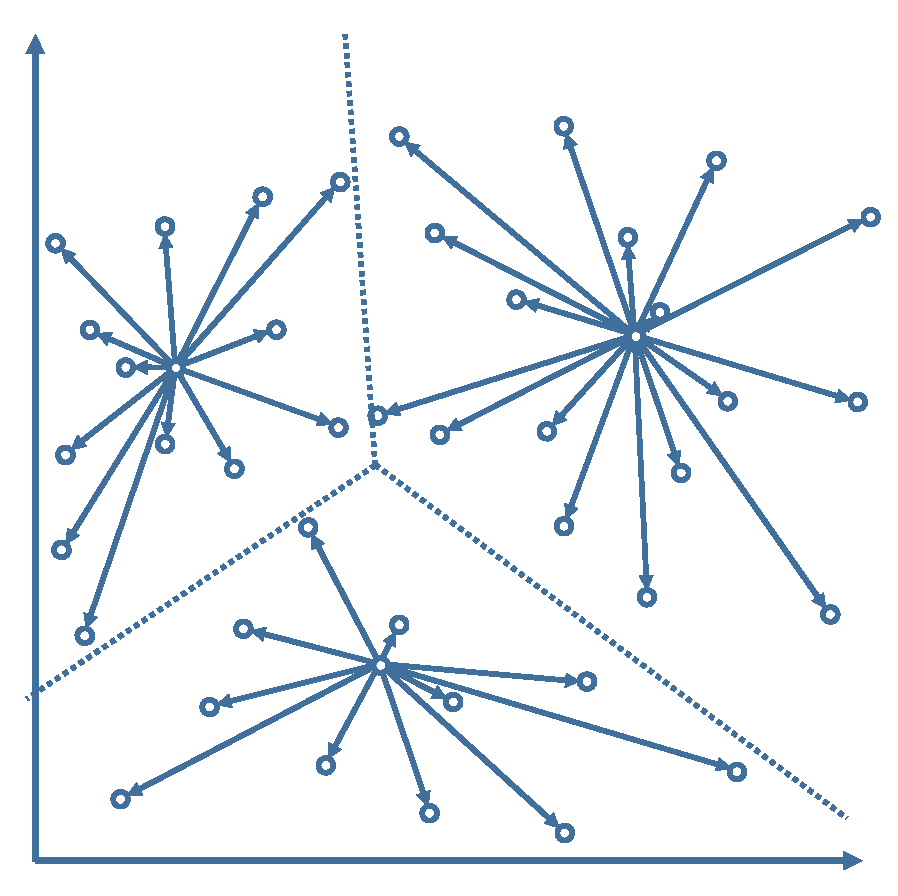
\includegraphics[height=40mm]{figure/vlad_5.eps}
   \hspace{1.6cm} (5) クラスタ毎にベクトル総和
  \end{center}
 \end{minipage}
%
 \begin{minipage}{0.33\textwidth}
  \begin{center}
   \includegraphics[height=40mm]{figure/vlad_6.eps}
   \hspace{1.6cm} (6) 特徴ベクトル化
  \end{center}
 \end{minipage}
%
\end{tabular}
\caption{VLADエンコーディング手順}
\label{fig:vlad_encoding}
\end{figure}

次に,特徴ベクトルの正規化を行う.本研究では,まず,特徴ベクトル$ \bm{v} $の各要素$ \bm{v_i} $に対して平方根によるパワー正規化を行い,$ L^2 $正規化を行った.さらに,$ \bm{v} $全体に対して$ L^2 $正規化を行った.

\newpage
%---------------------------------------------------------------------------------------------------
\section{識別器の学習}
動画像から得た特徴ベクトルを,複数クラスに分類するための識別器について述べる.
本システムでは,5つの行動カテゴリを識別するための学習モデルとしてSupport Vector Machine(SVM)を用いた.
SVMは,線形しきい素子を利用することで,特徴ベクトルの入力から直接帰属クラスを推定する識別関数を構築する手法である.一般化された識別関数は次式で表される.
%
\begin{equation}
{
  y(\bm{x})=\operatorname{sign}(\bm{w}^{\mathrm{T}}\bm{x}+w_0)
}
\end{equation}

ここで,$ \bm{x} $は入力される特徴ベクトル,$ \bm{w} $は重みベクトル,$ w_0 $はバイアスパラメータと呼ばれ,$ y(x) $はクラスに対応した2値のいずれかを取る.
また,重みベクトルとバイアスパラメータは,それぞれ識別面の方向と位置を決定する.
この時,識別対象である特徴ベクトルの高次元空間において,多数の学習データをクラス毎に上手く分離する識別面を探索することで,上記式のパラメータ$ \bm{w} $と$ w_0 $を推定することができる.
識別面を探索する際の評価基準は,各クラスに属する最近傍の学習サンプルとのユークリッド距離を最大化することである.

最も単純なSVMのモデルとして線形SVMがあり,特徴空間内における識別面は超平面となるが,現実には単純な超平面で完全分離できない場合が多い.
そのため,ある程度の識別誤差にペナルティを与え,外れ値として許容するソフトマージンや,サンプルデータを高次元空間へ非線形写像し,写像先の特徴空間で線形識別を行うカーネルトリックなどが導入される.
高い識別性能を達成するために,カーネルトリックを利用した非線形SVMが現在の主流となりつつあるが,計算コストの観点から本研究では利用せず,ソフトマージンを導入した線形SVMを利用する.
また,5つの行動を分類対象とするため,全ての2クラスの組み合わせにおいて識別関数を学習し,これらを統合したOne-versus-One分類器を構成することで,多クラス識別を行う.

%---------------------------------------------------------------------------------------------------
\section{識別評価}

%---------------------------------------------------------------------------------------------------
\subsection{評価法}
まず,各行動カテゴリ50シーケンスから,半数の動画をランダムサンプリングする.これらを学習データセットとし,Visual Words,PCAの主成分,SVMのパラメータを学習する.また,残り半数の動画をテストデータセットとし,特徴量計算,カテゴリ分類を行う.これを100回繰り返し,平均識別率を算出することで,3つの特徴表現手法について比較し,システムに最適な行動認識プロセスを検討する.

%---------------------------------------------------------------------------------------------------
\subsection{識別結果}
STIPを用いて検出した動画像の特徴点に対し,HOG,HOF,両者を連結したHOG/HOFの3種類の特徴記述子を用いて局所特徴を求めた.また,それぞれについてBag of Visual Words,Fisher Vector,VLADによるエンコーディングを行った.以下の図{\ref{fig:result_bovw}},図{\ref{fig:result_vlad}},図{\ref{fig:result_fisher}}では,各パターンにおいてVisual Wordsの数を10,20,50,100,200と変化させた場合のカテゴリ平均識別率の推移を示す.

%
\begin{figure}[htbp]
\begin{tabular}{cc}
%
  \begin{minipage}{0.5\textwidth}
    \begin{center}
      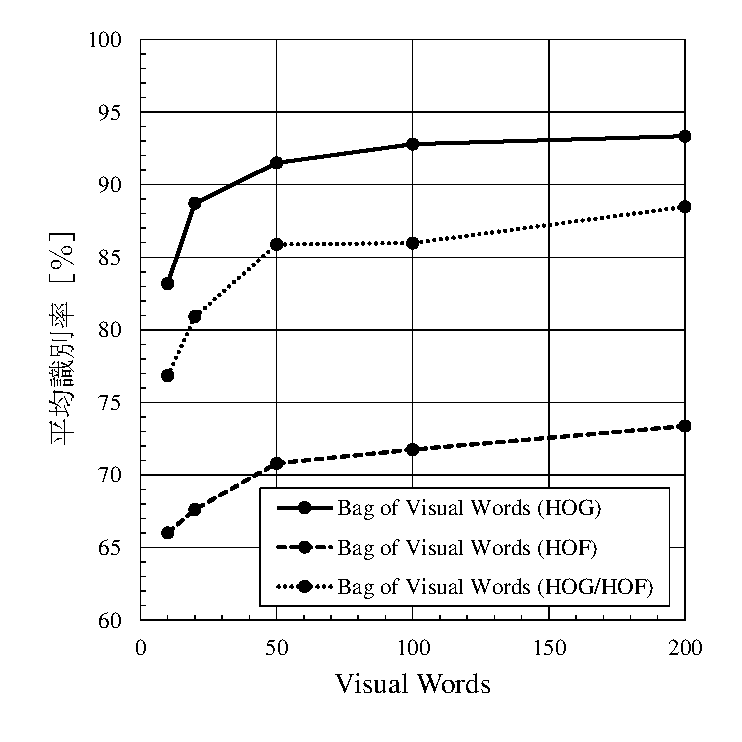
\includegraphics[height=70mm]{figure/result_bovw.eps}
      \vspace{-5mm}
      \caption{Bag of Visual Wordsの識別率}
      \label{fig:result_bovw}
    \end{center}
  \end{minipage}
%
  \begin{minipage}{0.5\textwidth}
    \begin{center}
      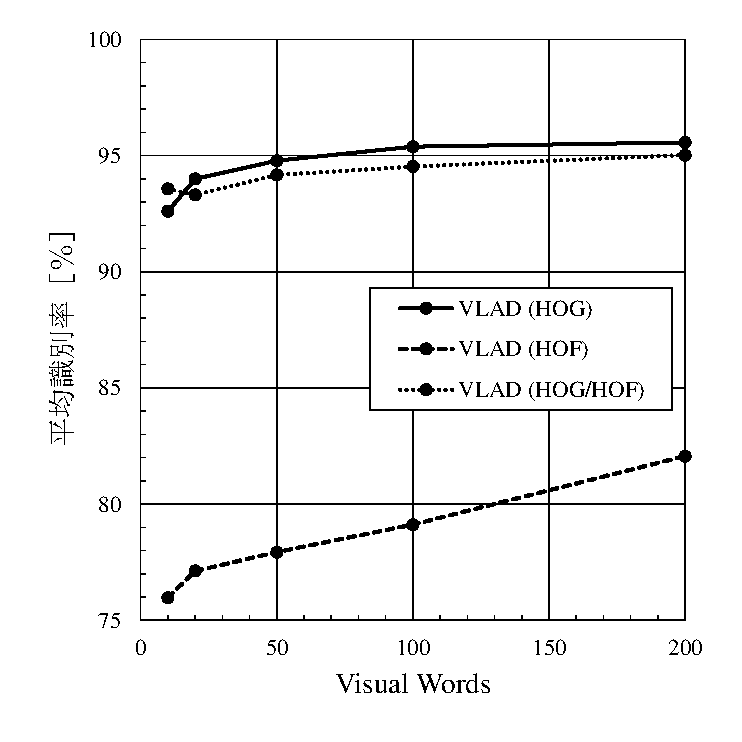
\includegraphics[height=70mm]{figure/result_vlad.eps}
      \vspace{-5mm}
      \caption{VLADの識別率}
      \label{fig:result_vlad}
    \end{center}
  \end{minipage}
%
\end{tabular}
\end{figure}
%
\begin{figure}[htbp]
\begin{tabular}{cc}
%
  \begin{minipage}{0.5\textwidth}
    \begin{center}
      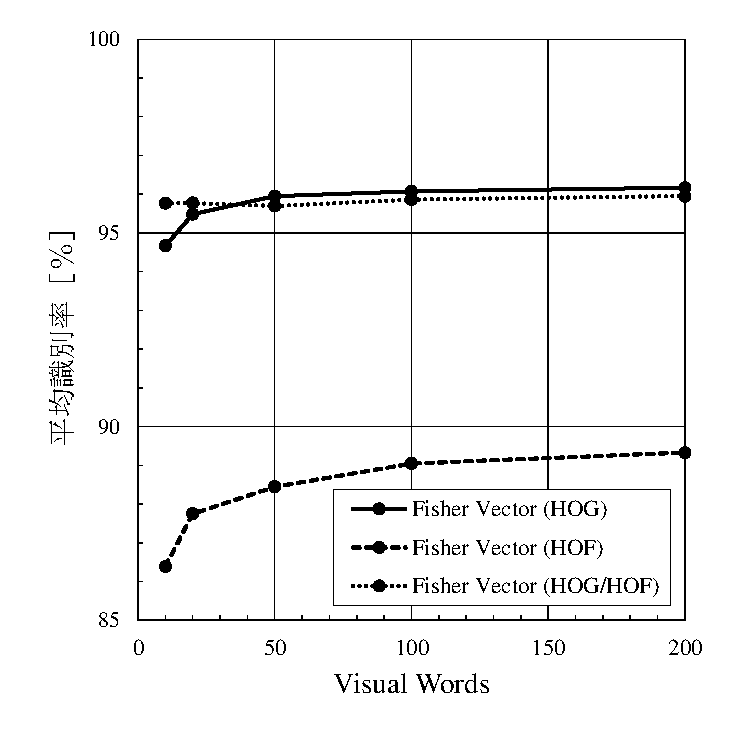
\includegraphics[height=70mm]{figure/result_fisher.eps}
      \vspace{-5mm}
      \caption{Fisher Vectorの識別率}
      \label{fig:result_fisher}
    \end{center}
  \end{minipage}
%
  \begin{minipage}{0.5\textwidth}
    \begin{center}
      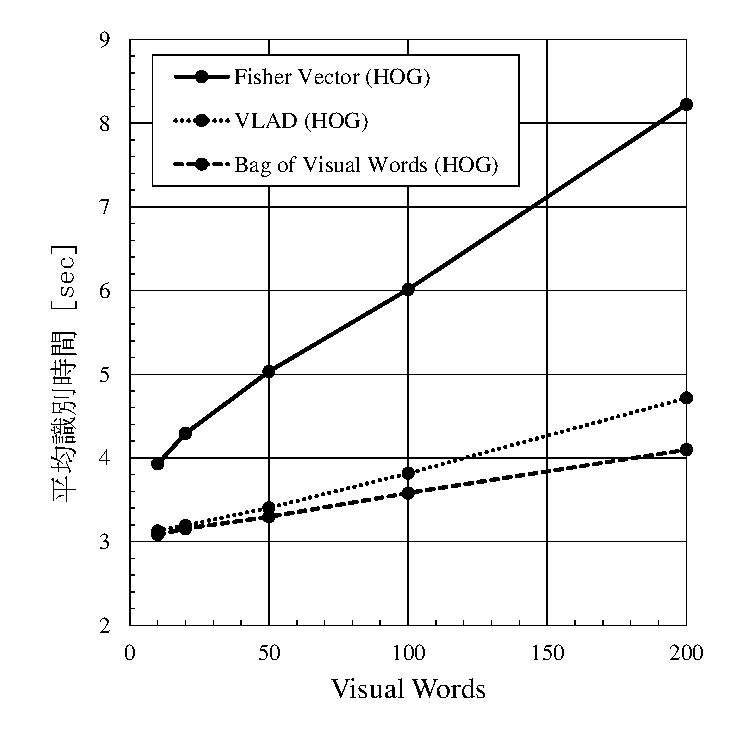
\includegraphics[height=70mm]{figure/result_time.eps}
      \vspace{-5mm}
      \caption{100回の試行における識別時間}
      \label{fig:result_time}
    \end{center}
  \end{minipage}
%
\end{tabular}
\end{figure}
%
\newpage

いずれのエンコーディング手法においても,特徴記述子としてHOGを用いた場合の識別率が最も高い傾向にある.
一方で,HOFを用いた場合の識別率は,HOGに比べて大きく下回っており,HOG/HOFを利用した場合も,ほとんどのVisual WordsにおいてHOGを下回る.
従って,動画像中の特徴点の動きよりも輝度勾配に基づく見えの特徴の方が,より精度の高い行動認識に寄与しうることが考えられる.
以降では,HOGを用いた場合に注目して比較を行う.

図{\ref{fig:result_time}}には,HOGを用いた場合の識別時間の推移を示した.
図によると,Visual Wordsの数に伴って,識別時間も一定の割合で増加しており,識別に最も時間を要するのはFisher Vectorである.これは,VLADとBag of Visual WordsがK-means法により求めた平均ベクトルでクラスタを表現するのに対し,Fisher Vectorでは,局所特徴にフィッティングさせた各ガウス分布によりクラスタを表現するため,Visual Wordsの計算コストの差が起因したものと考えられる.

また,識別率の推移に注目すると,いずれもVisual Wordsの増加に従って識別率が上昇し,Visual Wordsの数が100個の時にほぼ収束している.
ここで,各エンコーディング手法においてVisual Wordsの数が100個の場合に着目し,行動カテゴリ別の識別率を次の表{\ref{tb:result_table}}に示す.
%
{\newcolumntype{C}{>{\centering\arraybackslash}p{30mm}} 
\begin{table}[htbp]
  \begin{center}
  \makeatletter
  \def\@captype{table}
  \makeatother
  \caption{カテゴリ毎の識別率(HOG)}
  \label{tb:result_table}
    \begin{tabular}{CCCC} \bhline{1.2pt}
      \multicolumn{1}{c} {\multirow{2}{*}{行動}} & \multicolumn{3}{c}{識別率[%]} \\ \cline{2-4}
       & Bag of Visual Words & VLAD & Fisher Vector \\ \hline
      食事する & 97.0 & \bf{99.4} & 98.6 \\
      読書する & 90.6 & 94.0 & \bf{96.6} \\
      植木を注視する & 92.3 & 93.9 & \bf{94.0} \\
      ロボットを注視する & 91.2 & 93.7 & \bf{94.8} \\
      辺りを見回す & 92.8 & 95.9 & \bf{96.5} \\ \hline
      平均 & 92.8 & 95.4 & \bf{96.1} \\ \bhline{1.2pt}
    \end{tabular}
  \end{center}
\end{table}
}

ほとんどの行動カテゴリで,Fisher Vectorが最も高い識別率を示しており,平均識別率も最も高い.全体の傾向としては,1人称視点映像中の動きが少ない「植木を注視する」,「ロボットを注視する」といった行動カテゴリの識別率が低い.

以上を踏まえて,本システムでは,動画像の特徴記述子としてHOGを用い,Fisher Vectorによるエンコーディングを行う.また,Fisher VectorのVisual Wordsの数を100とする.

%---------------------------------------------------------------------------------------------------
\section{指示対象の推定法}
音声指示から複数候補が列挙された場合の行動情報による対象推定法に述べる.
本システムでは,TMSデータベースの物品情報の項目の一つ「タグ」を利用して,候補物品と認識された行動情報との関連度を比較する.タグ情報は,物品に関連するキーワードを羅列した項目である.例えば,お茶の入ったペットボトルには,「drink」,「tea」,「water」といった情報がタグとして登録される.
物品と行動情報の関連度は次のように求める.

まず,各行動情報にも表{\ref{tb:tags_for_activities}}で示すようなデータベースと同様のタグを複数割り当てておく.
物品候補が与えられると,各物品に登録されているタグとその時点の行動情報に結びつけられたタグとでマッチする個数をカウントし,その個数の大きい順から指示対象としての優先度を与えていく.
%
\begin{table}[htbp]
  \begin{center}
  \caption{各行動に関連するタグ情報}
  \label{tb:tags_for_activities}
    \begin{tabular}{cc} \bhline{1.2pt}
      行動 & タグ \\ \hline
      読書する & drink, coffee \\
      食事する & drink, tea \\
      植木を注視する & pot \\ \bhline{1.2pt}
    \end{tabular}
  \end{center}
\end{table}
\vspace{-10mm}

%---------------------------------------------------------------------------------------------------
\section{システム構成}
本節では,設計したシステムの構成についてを述べる.システムは,行動識別のリアルタイム性を考慮し,全体の処理をウェアラブル端末とサーバPCに分散した.また,TMS環境内での稼働を想定し,各処理ノードと通信はROSをフレームワークとして実装した.
%
\begin{figure}[htbp]
  \begin{center}
   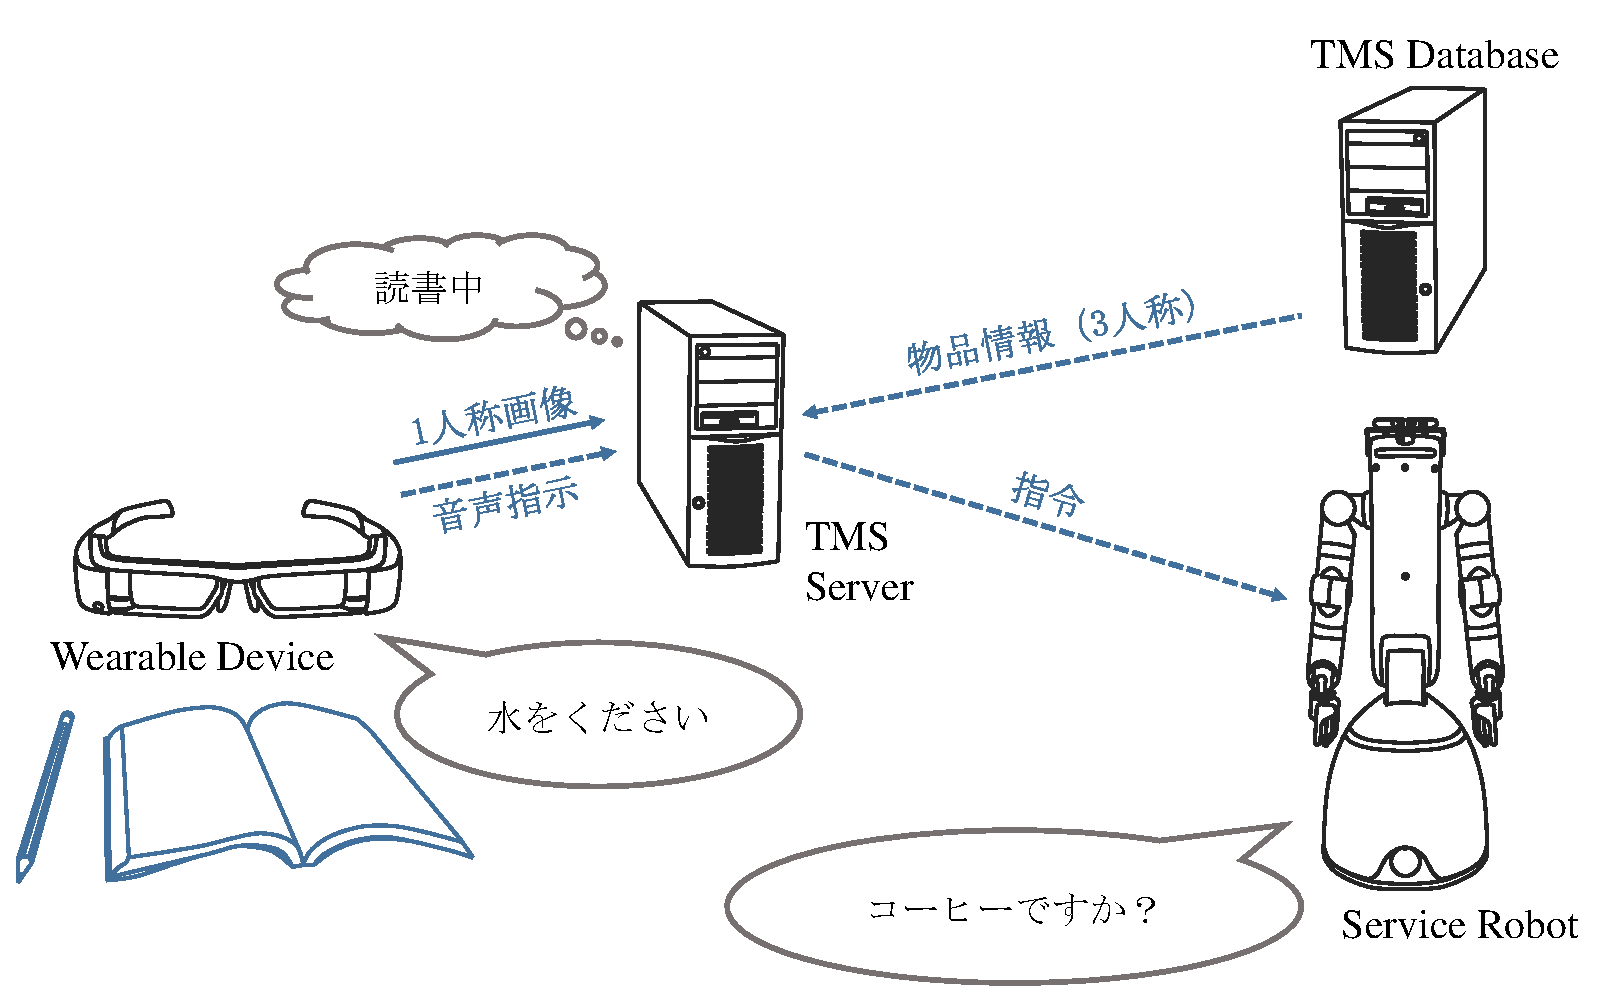
\includegraphics[height=80mm]{figure/system_2.eps}
   \caption{システムデザイン}
   \label{fig:system_2}
  \end{center}
\end{figure}

%---------------------------------------------------------------------------------------------------
\subsection{ウェアラブルカメラ}
本研究で使用するウェアラブルカメラMoverio BT-200AVはAndroid OSを搭載しており,ウェアラブルカメラとしての1人称視点画像取得に加えて,多様な機能を付加することができる.本システムでは,サービス要求生成に必要な1人称視点画像と音声指示の取得,システムユーザへの情報提示を行う.1人称視点画像は,搭載するカメラから取得した後,画像圧縮を施し,動画像のフレームレートに相当する一定周期でサーバに送信する.音声指示は,搭載するマイクから不定期に受け付け,認識できればサーバへの送信を行う.また,サーバの処理状況やサービスの実施状況を搭載ディスプレイから適宜提示する.

%---------------------------------------------------------------------------------------------------
\subsection{サーバPC}
サーバPCが担う処理は,受信する1人称視点画像から動画を生成し装着者行動を識別することと,システムユーザの音声指示に関連する物品候補情報を取得,それら候補を装着者行動に基づいてソートし,サービスロボットへ発話指令を送信することである.
%
\begin{itemize}
\setlength{\itemsep}{-5pt}
\item{ウェアラブルカメラから受信する1人称視点画像から動画像生成}
\item{動画像から特徴ベクトルを計算し,行動識別}
\item{ユーザの音声指示を受信し,その内容に関連する物品候補リストをTMSデータベースから取得}
\item{物品候補リストをその時点の行動情報に基づいて,ソート}
\item{サービスロボットへ発話指令を送信}
\end{itemize}

ウェアラブル端末から受信する1人称視点画像は,一定周期で固定バッファに格納し,空きが無くなった時点で行動認識を開始する.行動認識のプロセスは,バッファ内画像列からの動画像生成,STIPによる特徴検出と特徴抽出,PCAによる次元削減,局所特徴群のエンコーディング,SVMによる識別から構成される.また,システムユーザの音声指示は別スレッドから受け付け,指示内容に従ってその時点の行動情報を参照することで,適切な応答をサービスロボットに命令する.